% !TeX root = main.tex
% !TeX spellcheck = en-US
% !TeX encoding = utf8


\chapter{Results and Evaluation}
\label{chap:results}

All experiments and analyses were performed as previously described in \cref{chap:testing,chap:analysis}. 

\section{Part I - Choosing the Optimization Algorithm}
\label{chap:part1}
The results of the first experimentation part are very insightful and allow for a sound analysis of the most appropriate optimization algorithm to tune the parameters of the \gls{hsppbo} algorithm. Note that an evaluation of the quality of the solution itself and of the performance of the \gls{hsppbo} algorithm is not discussed in this first part. The solution quality is only used to compare the optimization methods. 

\begin{figure}[h]
	\centering
	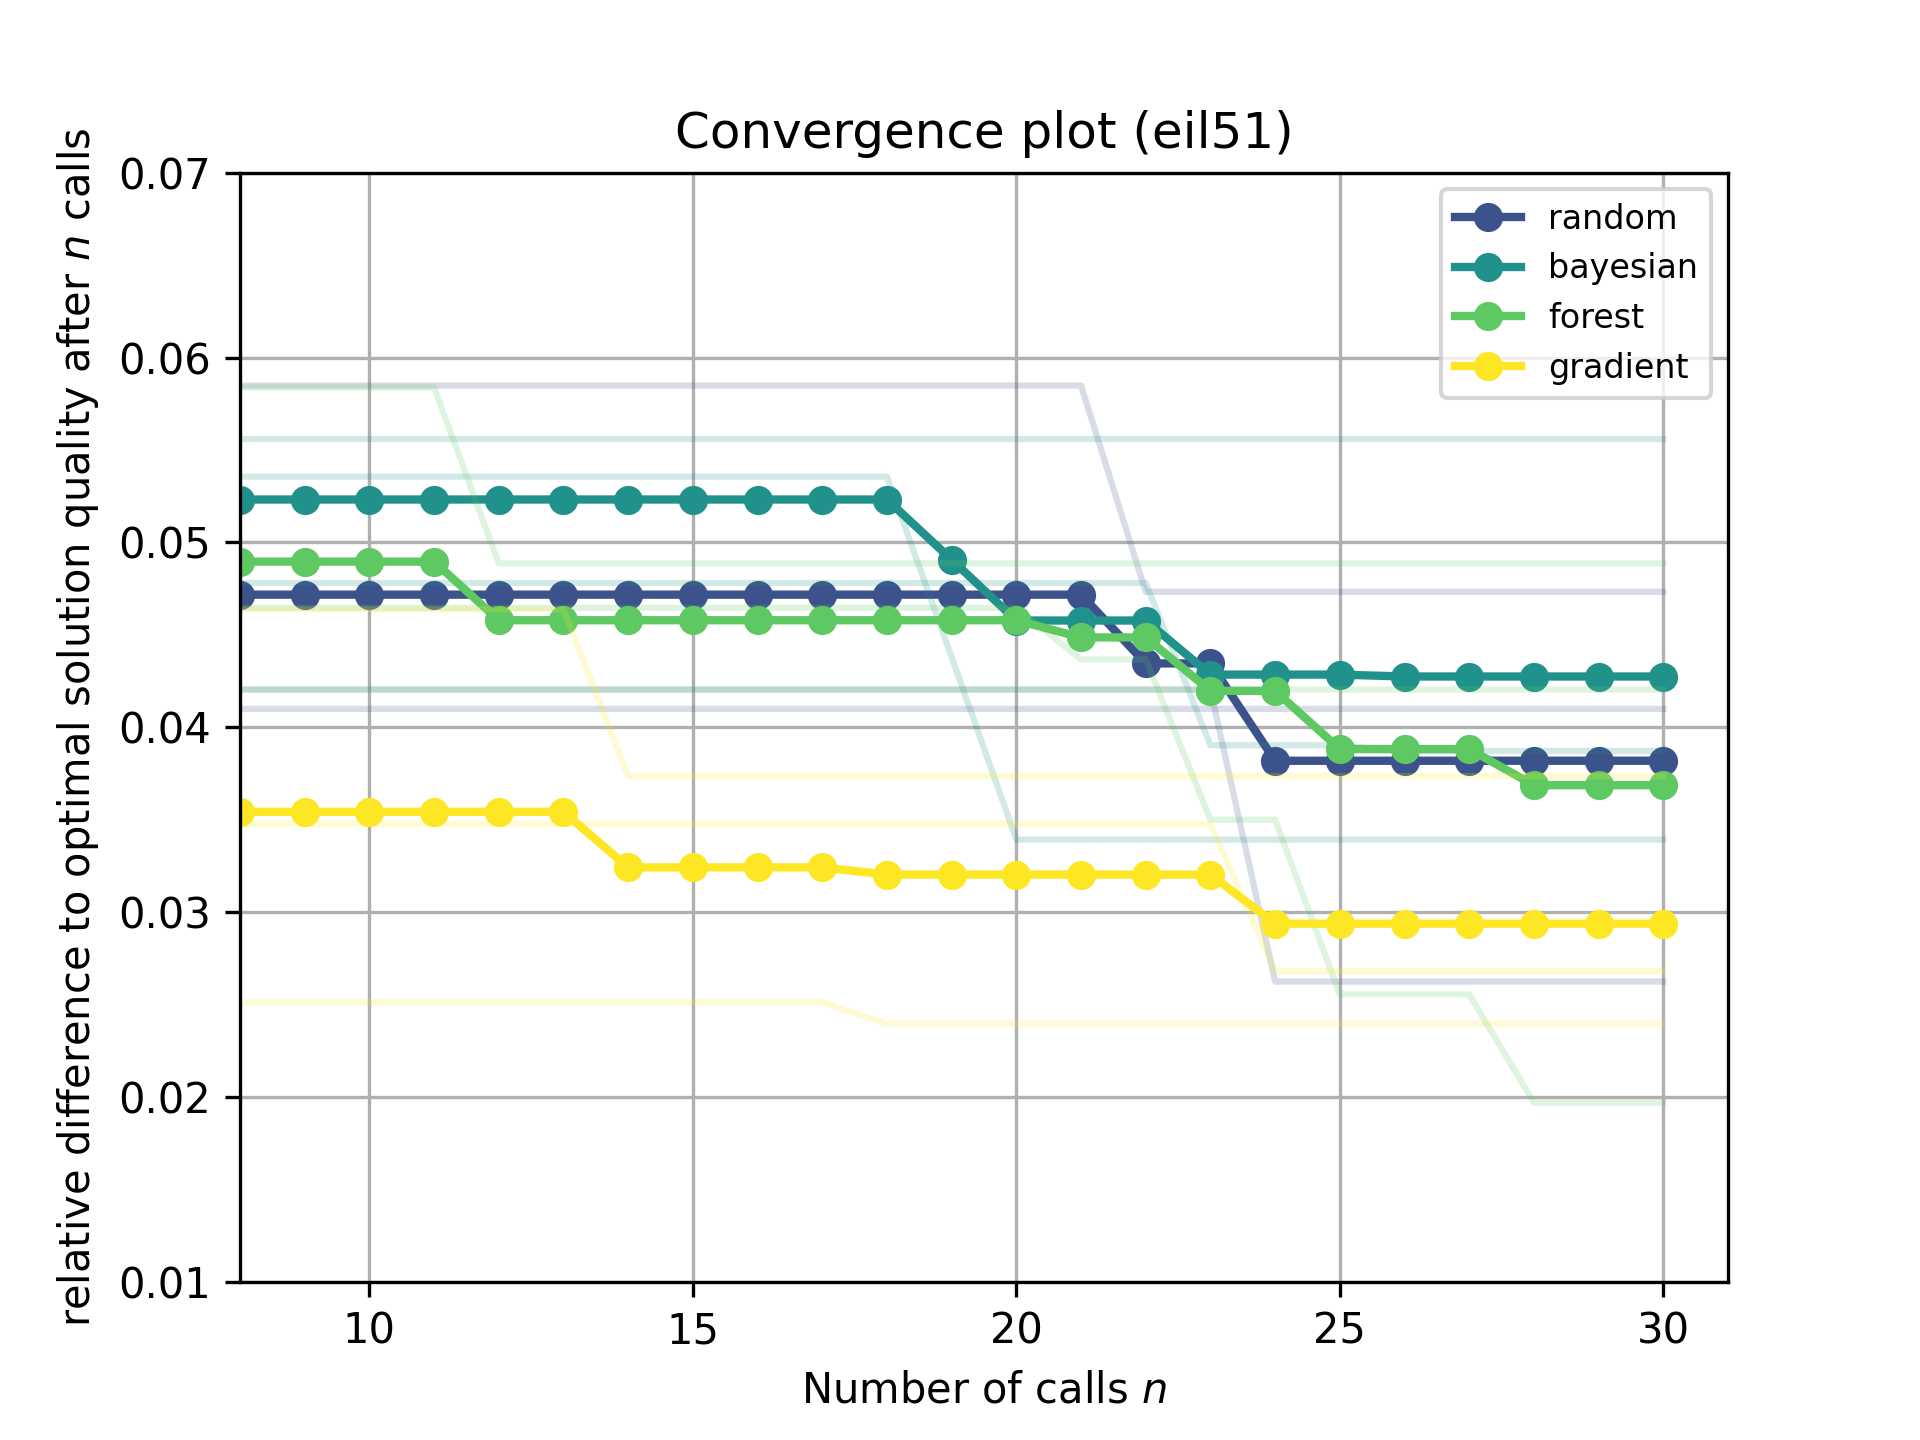
\includegraphics[width=0.75\textwidth]{results/part1/convergence_eil51.png}
	\caption[Convergence plot of \gls{tsp} instance \texttt{eil51}]{Convergence plot of \gls{tsp} instance \texttt{eil51}, comparing four different optimization algorithms.}
	\label{fig:convergence_eil51}
\end{figure}

First, the convergence plots of all five individual instances and their average are discussed. As explained in \cref{chap:an-part1}, these graphs show the minimum of the relative difference to the optimal solution $RPD$ up to each objective function call (\texttt{n\_call}). \cref{fig:convergence_eil51} shows this plot for the \texttt{eil51} \gls{tsp} instance. The bold, yellow line, which shows the average of the three \gls{gbrt} runs, indicates that this algorithm found the best solution over the course of the 30 objective calls. Except for a single run, where \gls{et} performed admirably, achieving a 2\% difference from the optimal solution, none of the other algorithms were able to come close to \gls{gbrt}. However, the average convergence behavior of all four algorithms seems to be very similar, with moderate improvements between objective calls 17 and 25. This behavior suggests that the first 10 sampling calls were sufficient to obtain a decent parameter configuration for the \texttt{eil51} instance. The specific runs (light colored lines) show that \gls{rs} and \gls{et} fluctuated the most in terms of initial solution quality and improvement over time. Although \gls{gp} produced the worst solutions out of all four algorithms, it still managed to achieve an average solution quality of almost 4\% after the full 30 \texttt{n\_calls}.

\begin{figure}[h]
	\centering
	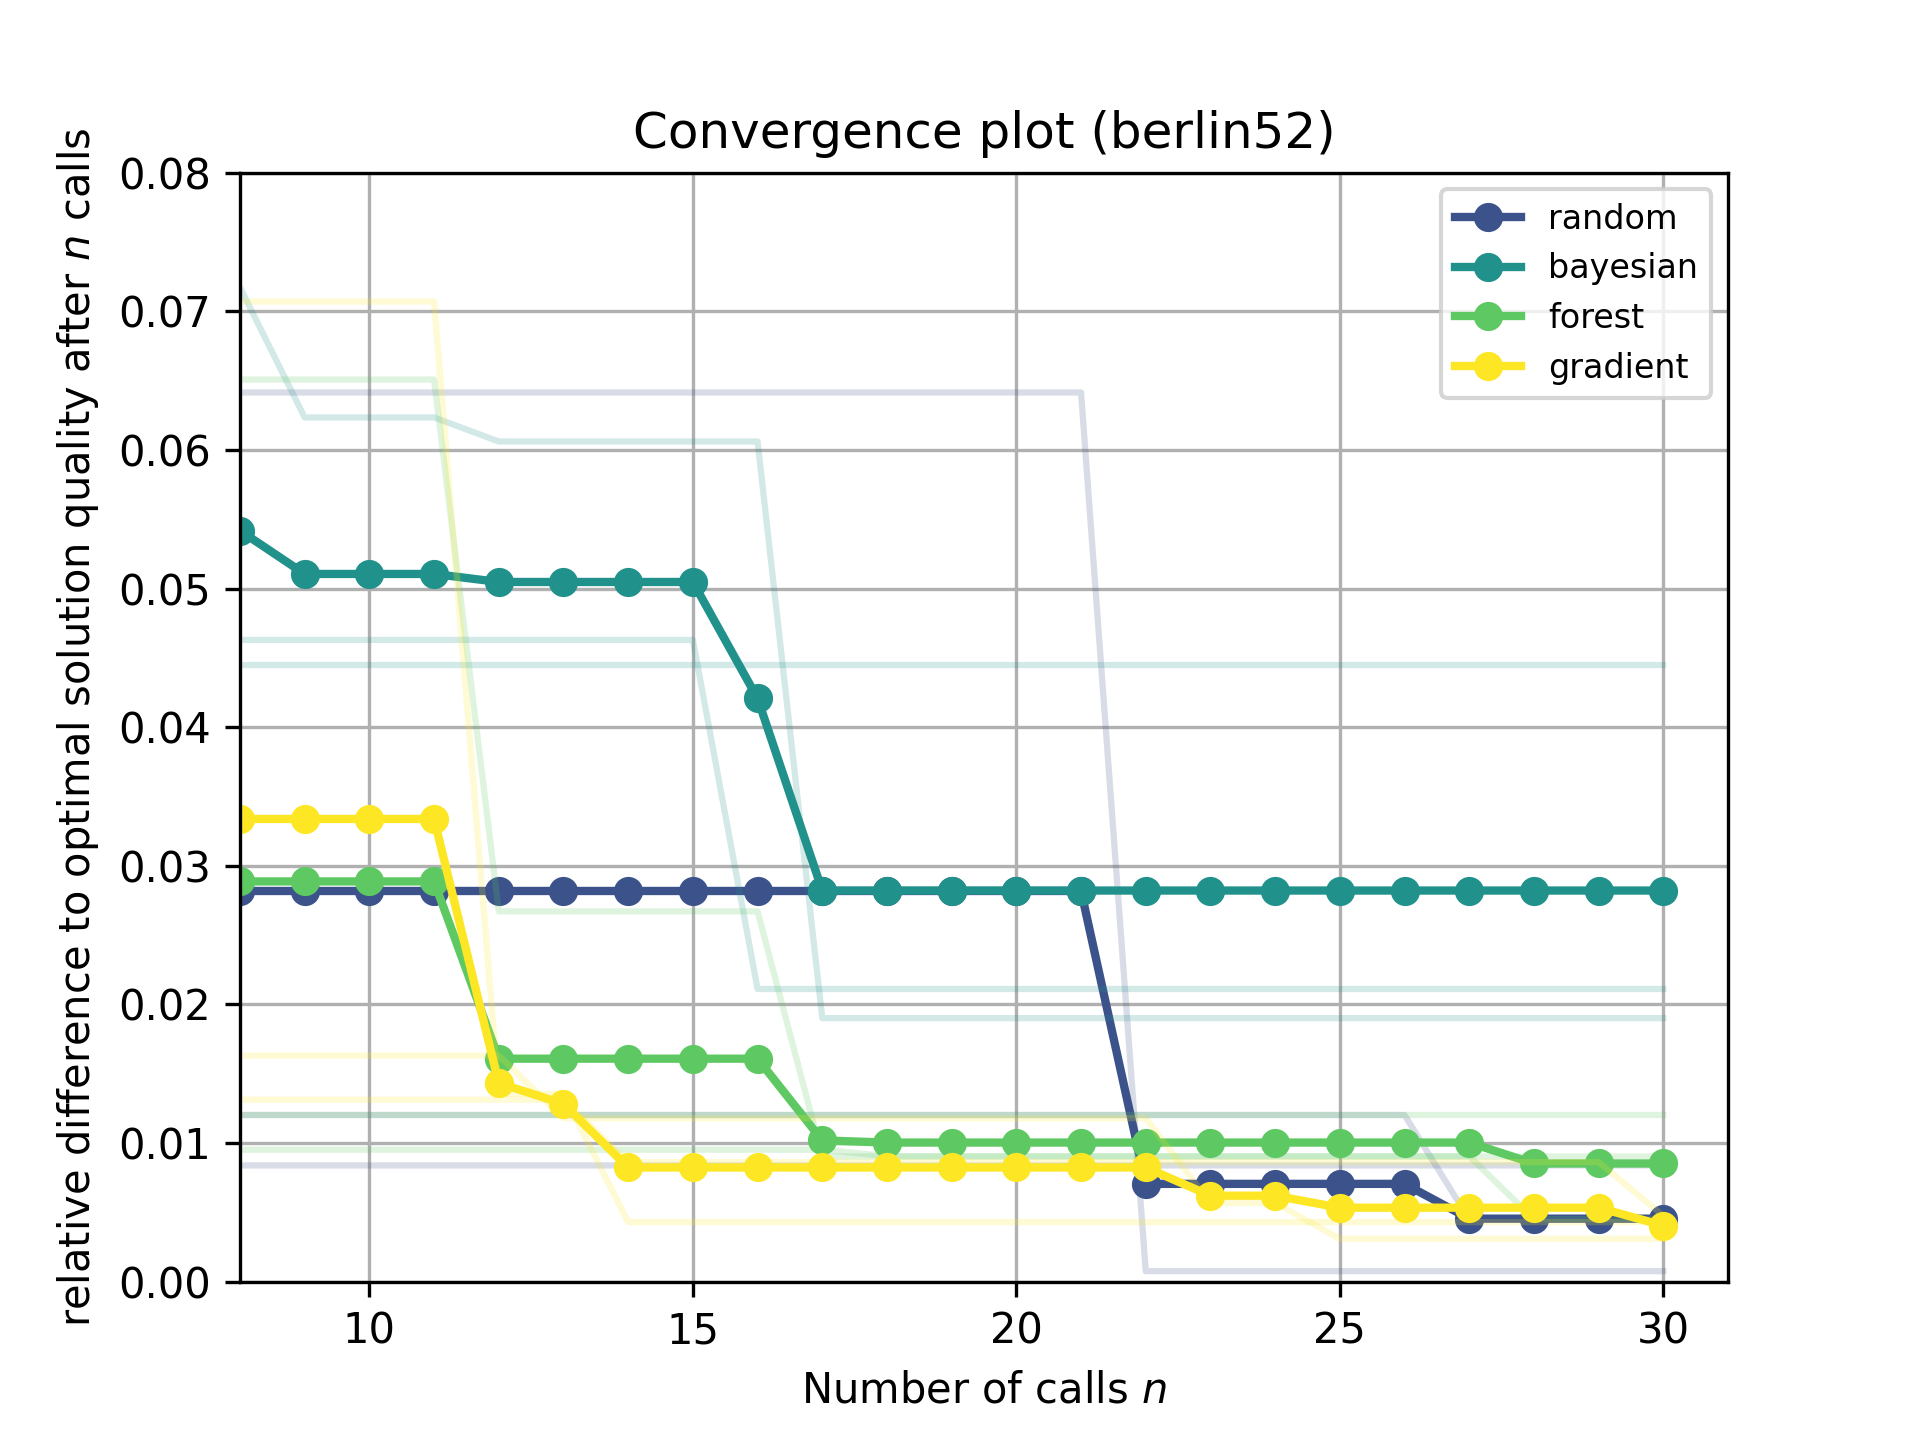
\includegraphics[width=0.75\textwidth]{results/part1/convergence_berlin52.png}
	\caption[Convergence plot of \gls{tsp} instance \texttt{berlin52}]{Convergence plot of \gls{tsp} instance \texttt{berlin52}, comparing four different optimization algorithms.}
	\label{fig:convergence_berlin52}
\end{figure}

The next instance is \texttt{berlin52}, whose convergence plot is shown in \cref{fig:convergence_berlin52}. Here, \gls{gp} continues to be the least well performing \gls{hpo} method, with a final average $RPD$ of only about 3\%, with one particular run reaching as low as $4.5\%$. All other methods achieved at least 2\% lower $RPD$ values, with \gls{rs} and \gls{gbrt} having an almost identical final $RPD$ of 0.5\%. 
However, \gls{gp} was able to improve its solution by a significant 2\% over the course of seven additional objective calls, suggesting that the algorithm was quickly making use of the now utilized, underlying model.
Due to the very random nature of \gls{rs}, some other individual runs started with a very high $RPD = 6.5\%$ and then, improved very abruptly after about 21 objective calls. The convergence behavior of \gls{rf} and \gls{gbrt} is quite similar and shows that both started with a good solution already at about 3\% for the tenth objective call, and then gradually improved up to objective call 17, analogous to \gls{gp}, but with less relative improvement. After that, only small gains in solution quality were achieved.

\begin{figure}[h]
	\centering
	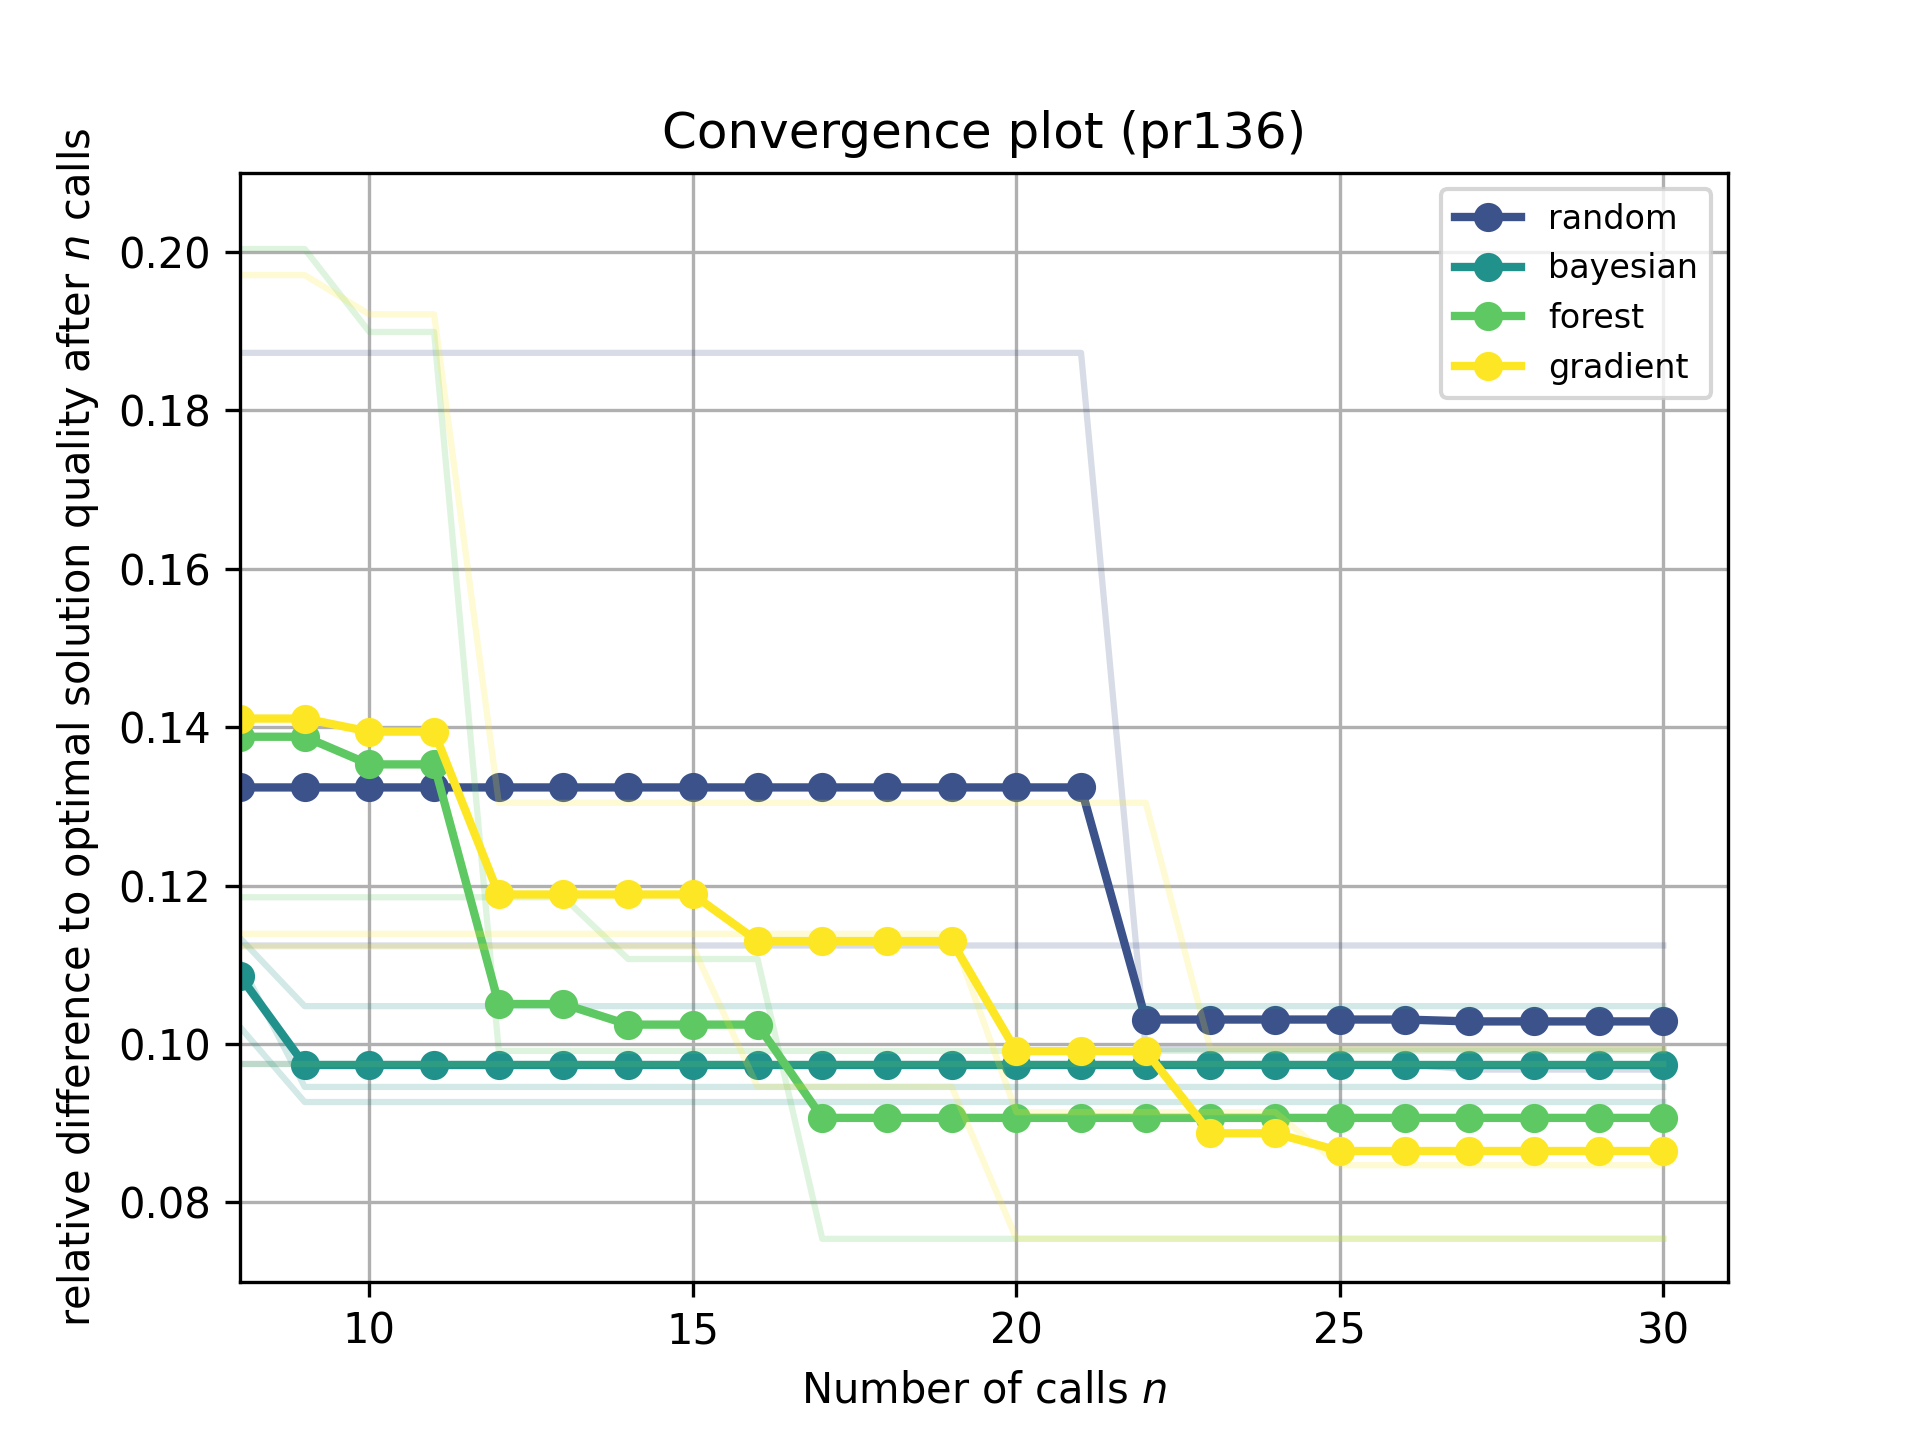
\includegraphics[width=0.75\textwidth]{results/part1/convergence_pr136.png}
	\caption[Convergence plot of \gls{tsp} instance \texttt{pr136}]{Convergence plot of \gls{tsp} instance \texttt{pr136}, comparing four different optimization algorithms.}
	\label{fig:convergence_pr136}
\end{figure}

The \texttt{pr136} \gls{tsp} instance, presented in \cref{fig:convergence_pr136}, continues the trend of \gls{gbrt} performing the best of the four optimization algorithms, albeit with a small lead of less than 0.5\% over the next best method, \gls{et}. Interestingly, \gls{gp} started with a considerably better initial sample at $RPD = 11\%$ after 10 objective calls, which gave it a head start, but also caused the algorithm to stagnate over the course of the remaining 20 calls. This might be due to the fact that Hammersley sampling was chosen only for this particular algorithm, or it could just be another random influence. \gls{et} and \gls{gbrt} gradually improved the most out of the four methods, with steep drops of around 2\% or more by the 23rd objective call. \gls{rs} rarely saw any meaningful improvement after the initial sampling, and the huge drop in average $RPD$ was due only to a single run that remained at a relatively poor value of $RPD = 18.8\%$ up until the 21st \texttt{n\_call}.

\begin{figure}[h]
	\centering
	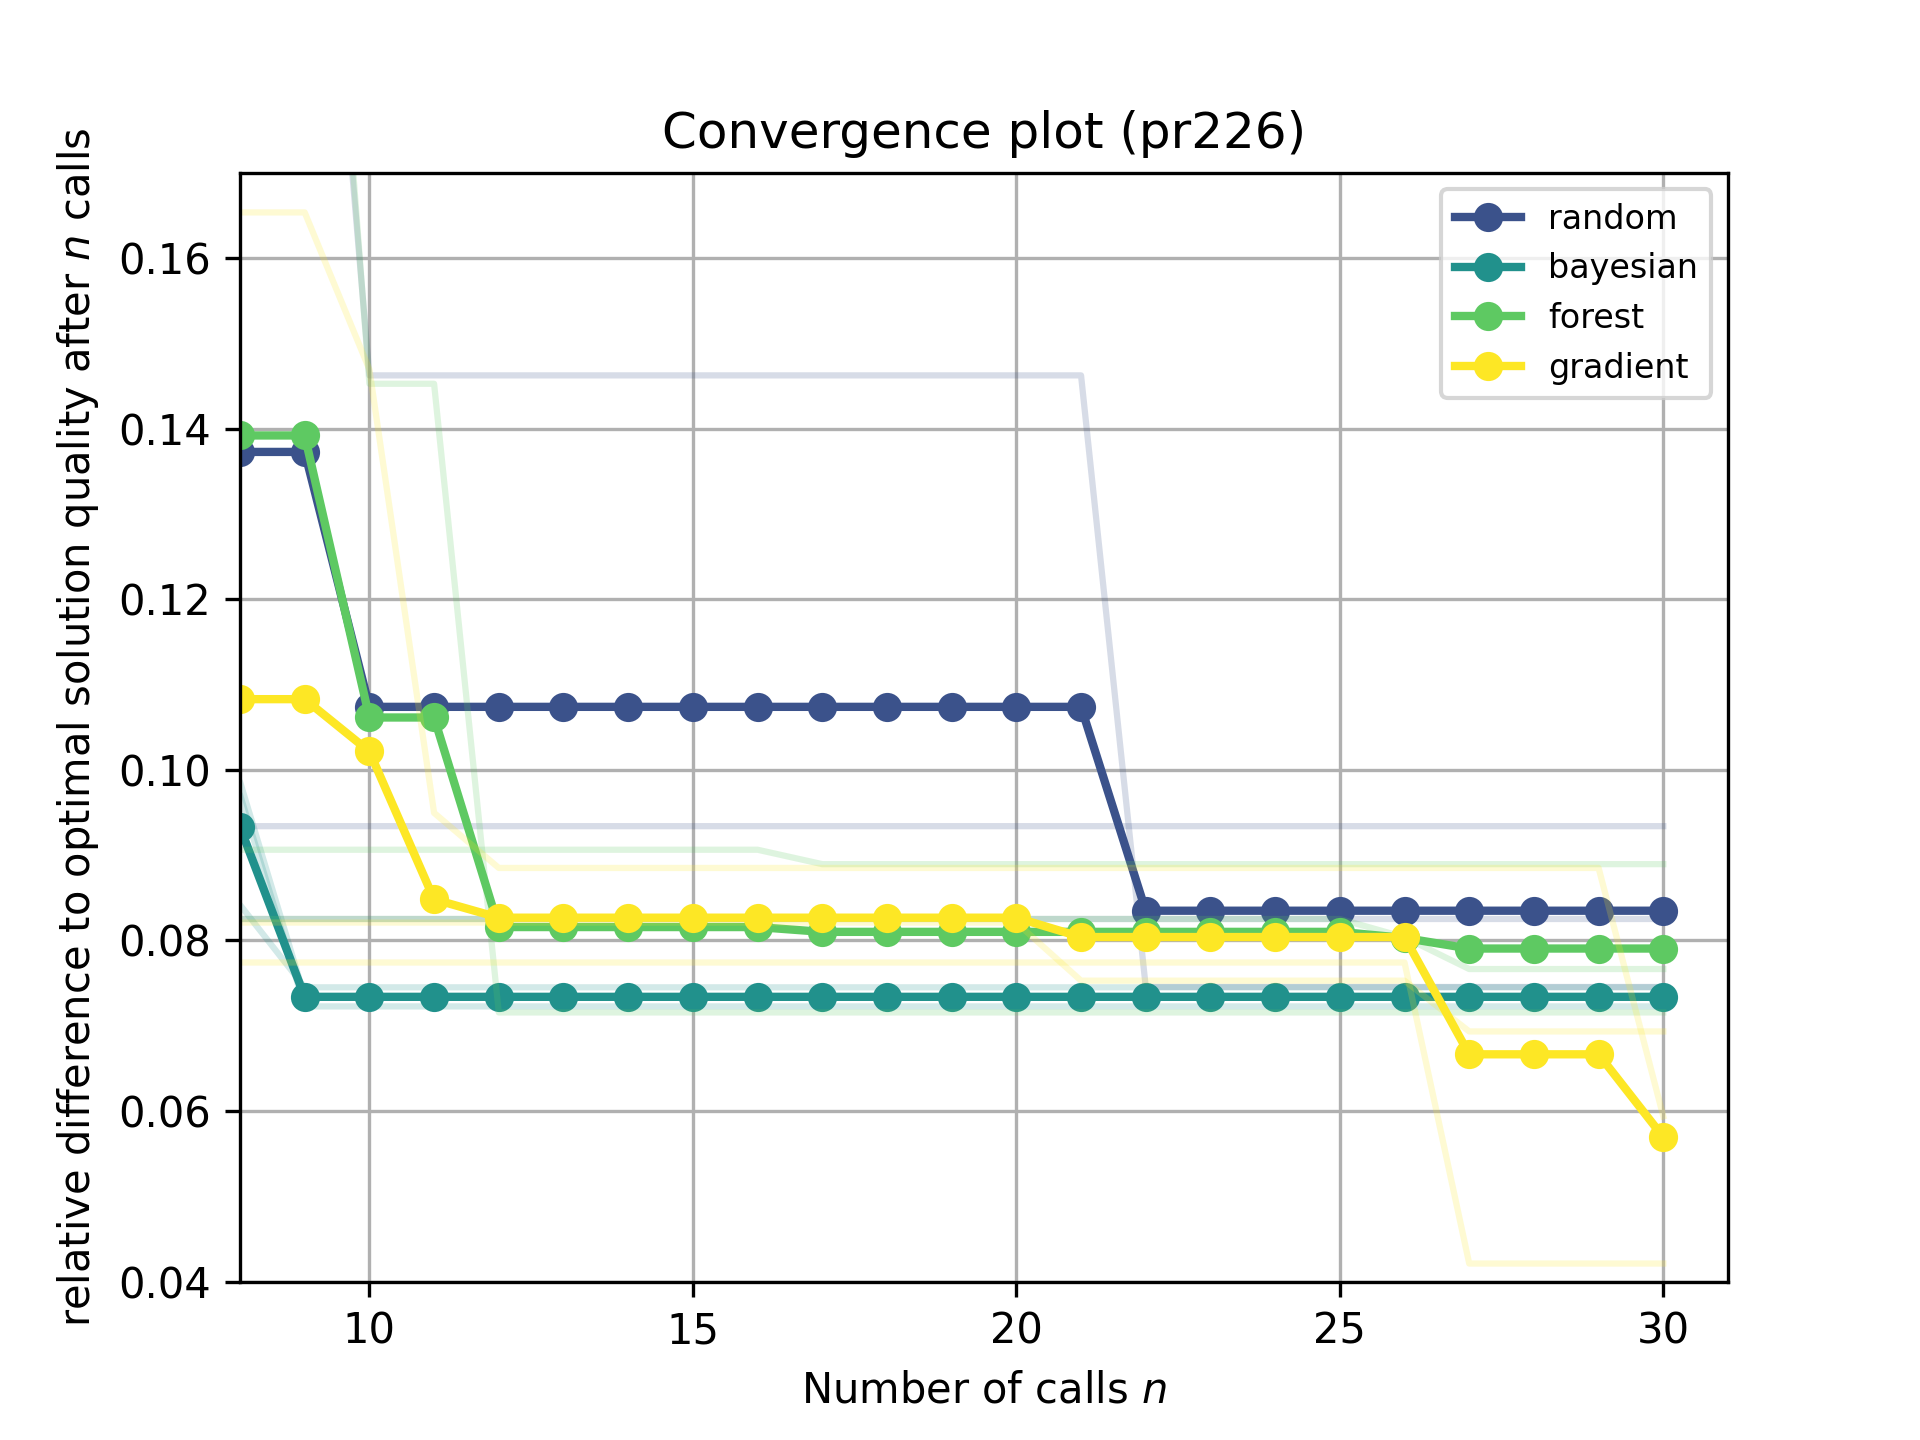
\includegraphics[width=0.75\textwidth]{results/part1/convergence_pr226.png}
	\caption[Convergence plot of \gls{tsp} instance \texttt{pr226}]{Convergence plot of \gls{tsp} instance \texttt{pr226}, comparing four different optimization algorithms.}
	\label{fig:convergence_pr226}
\end{figure}

The convergence plot in \cref{fig:convergence_pr226} for instance \texttt{pr226} again has \gls{rs} as the weakest method, with only small gains of about 2\% on objective call 22, bringing it to the average $RPD$ of the other algorithms. Some other single runs performed even worse. Contrary to the good performance of the other instances, this time \gls{et} starts its model training at 10 objective calls with a $RPD$ value almost the same as \gls{rs}, and only manages to significantly improve its parameters two \texttt{n\_calls} later. It then shows stagnant behavior at $RPD = 8\%$. Apart from the last five objective calls \gls{gbrt} showed a similar convergence behavior, improving by more than 2\% near the end, giving it the lead over \gls{gp}. This suggests that with larger instance dimensions and thus potentially more complex solutions, \gls{gbrt} benefits from more objective calls that improve the underlying model.
As with \texttt{pr136}, the initial sample of the Hammersley method potentially gave \gls{gp} a lead in solution quality, but then stagnated after the ninth call and was unable to improve its $RPD$ value of about 7.5\%.

\begin{figure}[h]
	\centering
	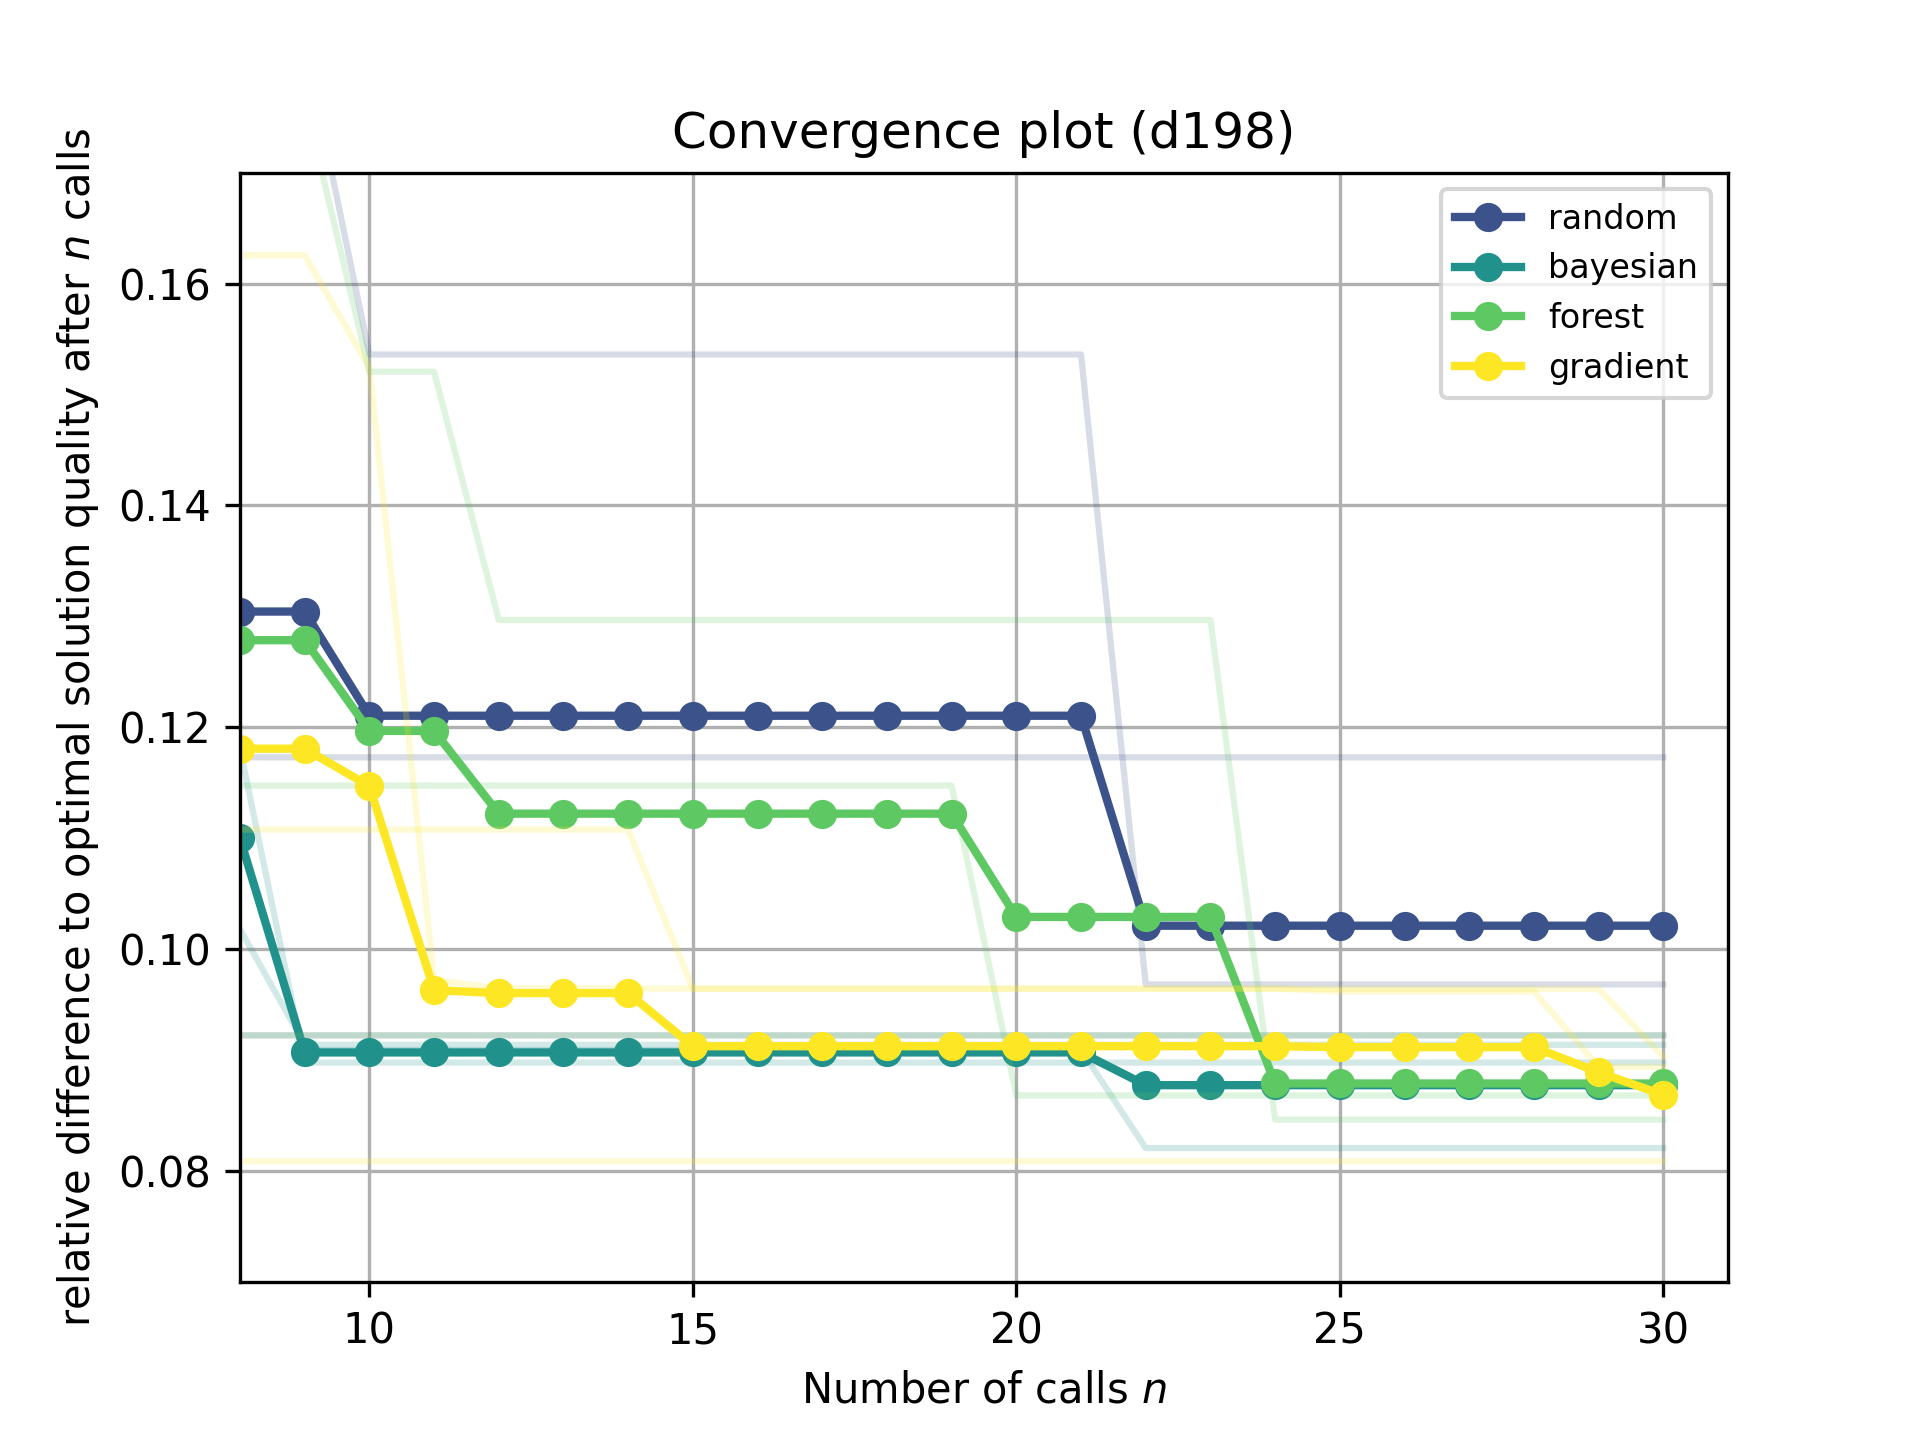
\includegraphics[width=0.75\textwidth]{results/part1/convergence_d198.png}
	\caption[Convergence plot of \gls{tsp} instance \texttt{d198}]{Convergence plot of \gls{tsp} instance \texttt{d198}, comparing four different optimization algorithms.}
	\label{fig:convergence_d198}
\end{figure}

The last \gls{tsp} instance, \texttt{d198}, confirms the observations of the previous instances, but this time all methods except \gls{rs} are within very close proximity of each other after the 24th objective call. Although \gls{gbrt} takes the lead in final relative solution quality with just under 9\%, it is not by much. Together with \gls{gp}, both methods managed to achieve considerable improvements up until the 15th objective call, after which they more or less stagnated. \gls{et} started with a similarly sub-optimal $RPD$ as \gls{rs} at objective call 10, but was able to improve steadily over the next 15 \texttt{n\_calls}. As expected at this point, \gls{rs} only managed to meaningfully improve in one run at objective call 21, still placing its final $RPD$ more than 1\% above the rest of the methods.

\begin{figure}[h]
	\centering
	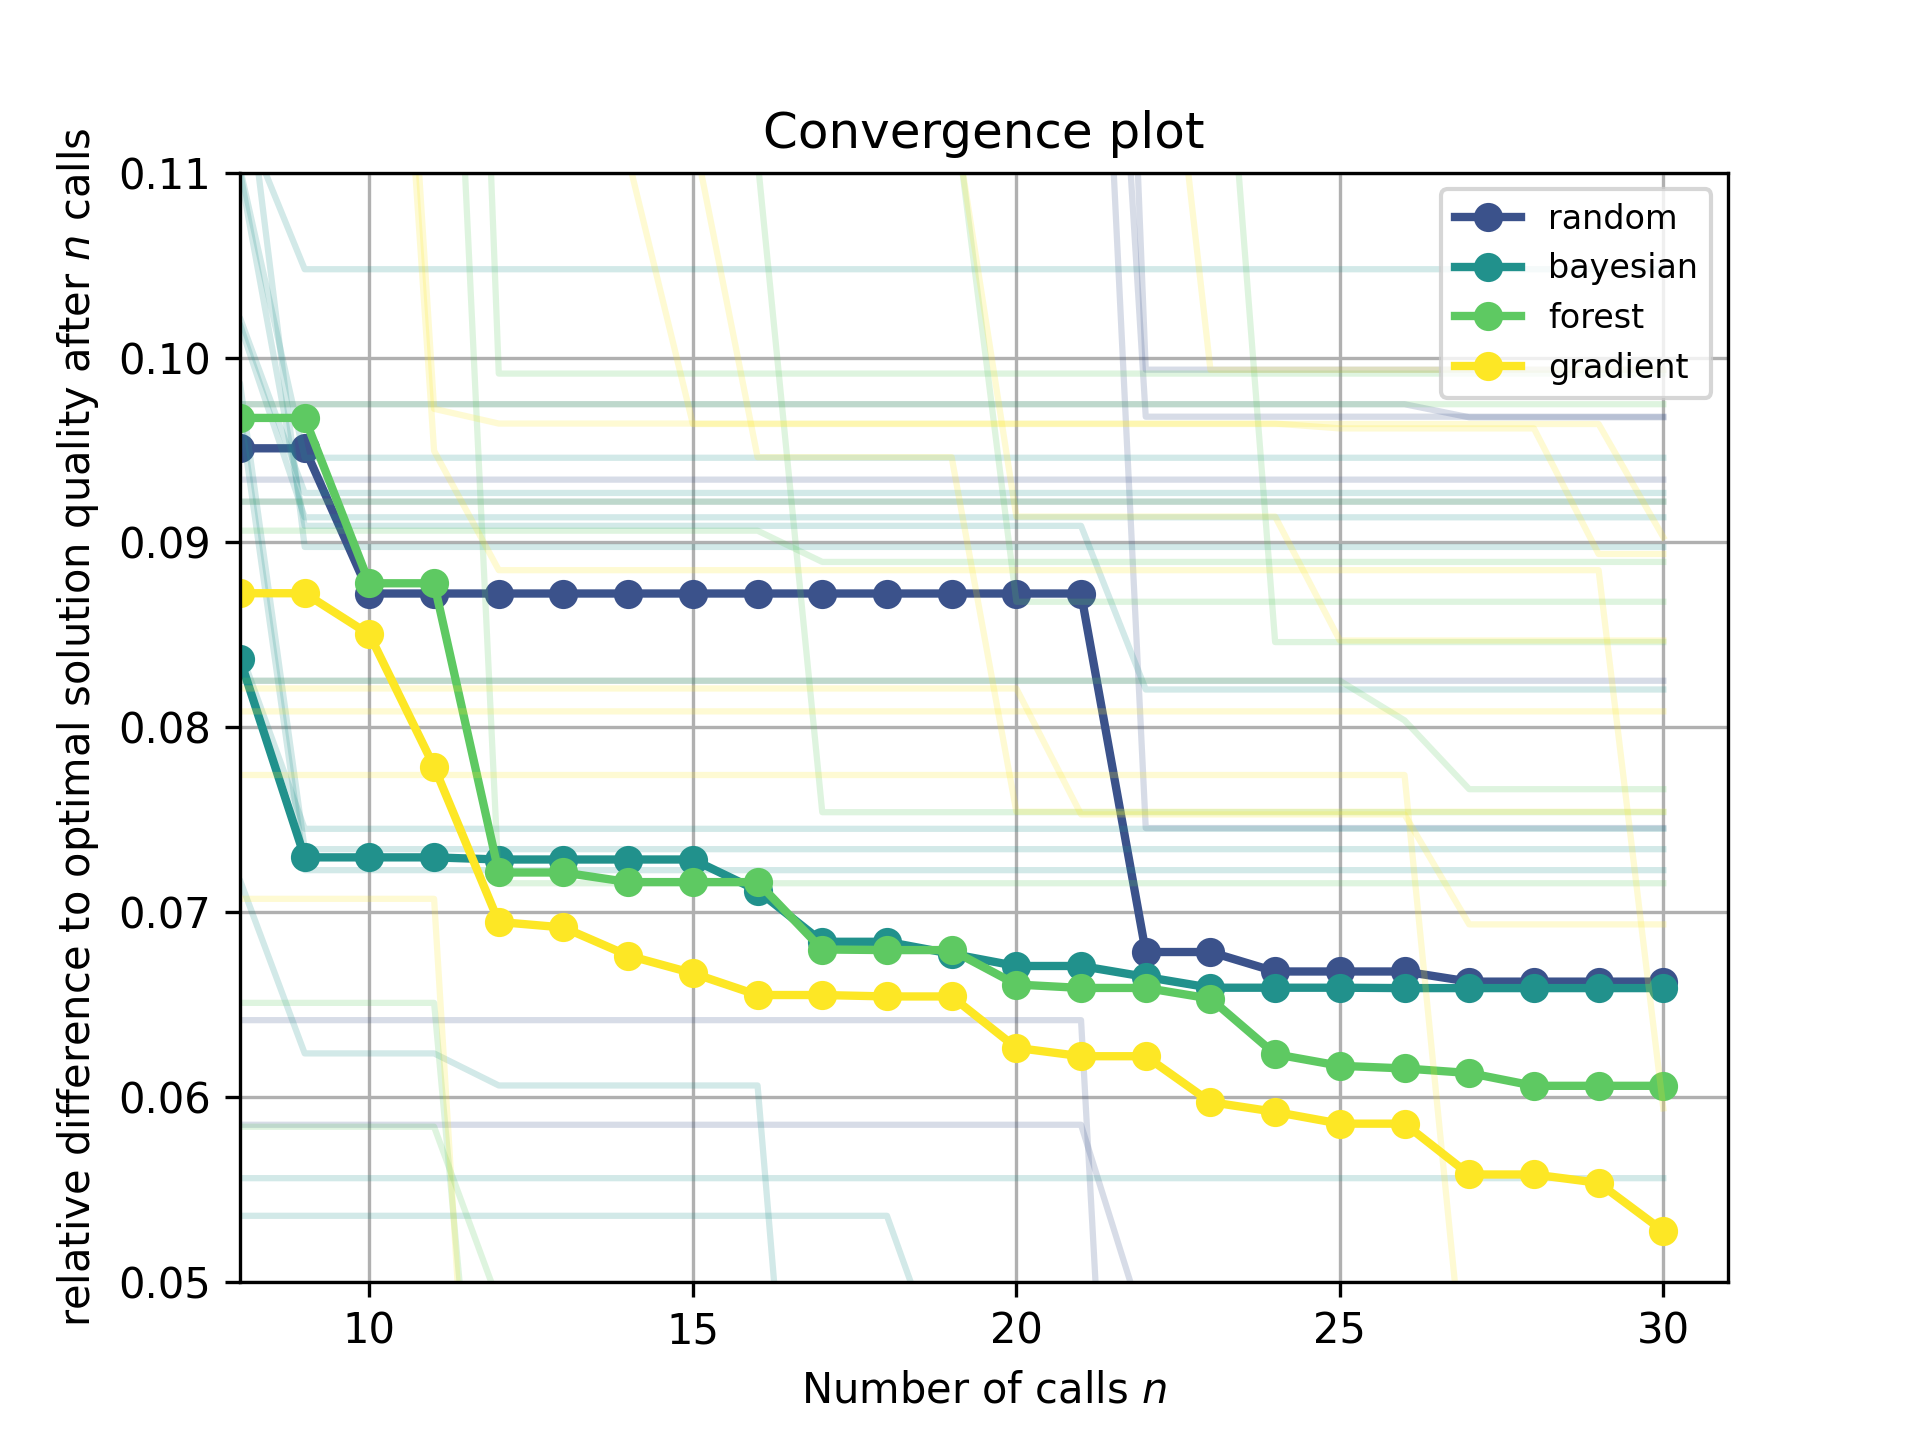
\includegraphics[width=0.75\textwidth]{results/part1/convergence_all.png}
	\caption[Convergence plot of the average over five \gls{tsp} instances]{Convergence plot of the average over five \gls{tsp} instances \texttt{eil51, berlin52, pr136, pr226, d198}, comparing four different optimization algorithms.}
	\label{fig:convergence_all}
\end{figure}

Lastly, the average convergence plot aggregates the runs of all five instances. Since \gls{gbrt} is the best performing method out of all the individual comparisons, its average convergence behavior emphasizes this by giving it a lead in final $RPD$ of about 1.5\% over the next best method, \gls{et}. Both methods show similar convergence behavior over the entire runtime, with large improvements in the first few objective calls, and small, but steady (almost linear) improvements thereafter. The behavior of \gls{gp} is not very different from previous descriptions, and is mainly distinguished by its better initial $RPD$ value, which reinforces the proposed relationship with the Hammersley sampling method. After this initial lead, the algorithm almost stagnates, and after the 22nd objective call, it converges to the trajectory of \gls{rs}.

\begin{table}[h]
	\centering
	\caption[The \gls{auc} and $RPD_{min}$ for all optimization runs]{The \gls{auc} and minimum relative solution quality at the last objective call ($RPD_{min}$) of all optimization runs for each method and instance, and for the mean over all instances.}
	\label{tab:part1-stats}
	\begin{tabular}{l c c c  c  c  c }
		 \hline
		~ & \multicolumn{2}{c}{eil51} &  \multicolumn{2}{c}{berlin52} &  \multicolumn{2}{c}{pr136} \\
		\cmidrule(lr){2-3} \cmidrule(lr){4-5} \cmidrule(lr){6-7}
		~ & \gls{auc} & $RPD_{min}$ & \gls{auc} & $RPD_{min}$ & \gls{auc} & $RPD_{min}$ \\ \noalign{\hrule height 1pt}
		RS & 0.830 & 0.026 & 0.347 & 0.001  & 2.266 & 0.097 \\
		GP & 0.900 & 0.034 & 0.650 & 0.019 & 1.850 & 0.093 \\ 
		ET & 0.819 & 0.020 & 0.227 & 0.005 & 1.809 & 0.075 \\ 
		GBRT & 0.601 & 0.024 & 0.159 & 0.003 & 1.948 & 0.075 \\ \noalign{\hrule height 1pt}
	\end{tabular}
	\bigskip\\
	\begin{tabular}{l  c  c  c  c  c  c}
	   \hline
		~ & \multicolumn{2}{c}{pr226} & \multicolumn{2}{c}{d198} & \multicolumn{2}{c}{mean}\\
		\cmidrule(lr){2-3} \cmidrule(lr){4-5} \cmidrule(lr){6-7}
		~ & \gls{auc} & $RPD_{min}$ & \gls{auc} & $RPD_{min}$ & \gls{auc} & $RPD_{min}$ \\ \noalign{\hrule height 1pt}
		RS &  1.837 & 0.075 & 2.139 & 0.092 & 1.484 & 0.058\\ 
		GP & 1.394 & 0.072 & 1.698 & 0.082 & 1.298 & 0.060\\
		ET & 1.547 & 0.072 & 1.940 & 0.085 & 1.268 & 0.051\\ 
		GBRT & 1.497 & 0.042 & 1.745 & 0.081 & 1.190 & 0.045\\ \noalign{\hrule height 1pt}
	\end{tabular}
\end{table}

Regarding the visually observable convergence behavior of the four optimization methods, we can also look at the \glsfirst{auc} of the plots and the minimum/best relative solution quality obtained, i.e. the $RPD$ value at $\texttt{n\_call} = 30$, hereafter called $RPD_{min}$. This data is presented in \cref{tab:part1-stats}, averaged over all available optimizer runs, for all five instances, and their mean.
In this context, a low \gls{auc} value indicates that the optimization algorithm found a well-performing parameter set, and therefore a low $RPD$, in a short time, i.e., few objective calls. However, the comparatively lowest \gls{auc} does not necessarily mean that it also found the lowest $RPD_{min}$ value among all algorithms. Thus, both values are discussed for each instance to determine how fast each algorithm converged to its best solution. For the \texttt{eil51} \gls{tsp} instance, \gls{gbrt} has by far the lowest \gls{auc} of 0.601. Paired with the second best $RPD_{min} = 2.4\%$, this method continues its favorable performance from the convergence plots. With a 0.4\% improvement in $RPD_{min}$ over \gls{gbrt}, \gls{et} was the second fastest to convergence to this final solution. \gls{gp} delivered the worst performance in this instance.

The \texttt{berlin52} instance implies a similar behavior, with \gls{gbrt} leading in convergence speed with the lowest \gls{auc}. However, as discussed in the corresponding convergence plot, \gls{rs} managed to find the best solution out of the four methods, with $RPD_{min} = 0.1\%$, outperforming \gls{gbrt} by 0.2\%. Again, \gls{gp} shows the worst performance, this time with an \gls{auc} of $0.650$, almost twice as high as its direct competitor \gls{rs} with $0.347$. \gls{et} is again the second fastest converging algorithm after \gls{gbrt}, with an almost equally good $RPD_{min} = 0.5\%$.

The results for \texttt{pr136} show an equal best $RPD_{min} = 7.5\%$ for \gls{gbrt} and \gls{et}, and an almost equal \gls{auc} for \gls{gp} and \gls{et}. Therefore, in this instance, \gls{et} outperforms \gls{gbrt} as the best converging algorithm. Interestingly, even \gls{gp} achieves a better \gls{auc} of $1.850$ than \gls{gbrt}, albeit with a worse minimum relative solution quality, which is more in line with \gls{rs}.

\texttt{pr226}, the largest \gls{tsp} instance out of the five tested in this part of the experimentation discussion, continues the improvement of \gls{gp} in terms of \gls{auc}, resulting in the best value out of all four algorithms, with a solid 7\% difference compared to the next best algorithm, \gls{gbrt}, which itself, was able to achieve the best $RPD_{min}$ at 4.2\%. \gls{rs} continues to perform worse as the instance dimension increases, which could be an opposite trend for the convergence speed of \gls{gp}.

The last \gls{tsp} instance, \texttt{d198}, confirms this implication, resulting in \gls{gp} again being the best algorithm in terms of \gls{auc}, and the second best in terms of $RPD_{min}$ at 8.2\%. This suggests, that this algorithm could benefit from larger, more complex instances, perhaps even from stronger clustering, as the latter two instances were categorized. \gls{gbrt} achieved the best $RPD_{min}$ value at 8.1\% and the second best \gls{auc}, which is only 2.7\% higher than the value of \gls{gp}. In this instance, the performance of \gls{et} was comparatively underwhelming, being closer to the \gls{auc} value of \gls{rs} than to the other two methods.

Finally, the mean results confirms that \gls{gbrt} was the algorithm that converged the fastest ($\gls{auc} = 1.19$) to the best performing parameter set ($RPD_{min} = 4.5\%$). Even in later, higher dimensional  instances, it performed at least the second best or better, implying good search consistency across the parameter space. \gls{et} obtained better solutions for the three smaller instances, resulting in lower averages compared to \gls{gp}, which showed the opposite trend, improving with higher problem dimension.

\begin{figure}[h]
	\centering
	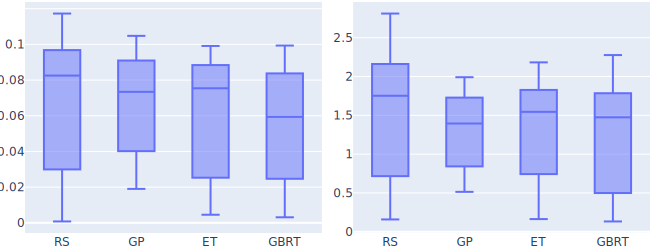
\includegraphics[width=\textwidth]{results/part1/convergence_stats_boxplot.svg}
\captionsetup[subfigure]
{skip=-8pt}
		\hfill
		\subcaptionbox{Relative difference to optimal solution quality at last the objective call ($RPD_{min}$) for all runs and instances.\label{fig:convergence_stats_boxplot_rpd_min}}[.45\linewidth]{\hfill}
		\hfill
		\subcaptionbox{\Glsfirst{auc} of solution quality convergence graph.\label{fig:convergence_stats_boxplot_auc}}[.45\linewidth]{\hfill}

	\caption[Statistical box plots illustrating convergence plots]{Statistical box plots illustrating the data of all five individual convergence plots and their individual runs.}
\label{fig:convergence_stats_boxplots}
\end{figure}

\Cref{fig:convergence_stats_boxplots} shows statistical box plots for both of the metrics from the table over all runs and data from all problem instances combined. This visualization is also used to evaluate the consistency across all four optimization methods, which was previously only implied by their average or best-case performance. However, this is not normalized by instance, so the absolute values and differences, as with the mean from the previous table, might not be as expressive. Nevertheless, since all four algorithms are affected by this bias, qualitative statements are still possible.

The dispersion of $RPD_{min}$ in \cref{fig:convergence_stats_boxplot_rpd_min} implies that \gls{gp} reached its solution most consistently at around its median of 7.5\%, but also never reached the same minimum as the other three algorithms. \gls{rs}, on the other hand, was the most unreliable method, with its maximum and minimum being far of from the upper and lower quartiles, respectively. It also has the highest median at about 8\%. \gls{gbrt} and \gls{et} share similarities in their \gls{iqr} and minimum/maximum values, with \gls{gbrt} having a slightly smaller dispersion. However, they differ tremendously in their median, with \gls{et} having a value almost 2\% higher than \gls{gbrt}, which means that although both their solution consistency is not ideal, \gls{gbrt} still obtained the best final solution out of all algorithms.

The box plots for the \gls{auc} (\cref{fig:convergence_stats_boxplot_auc}) show similar consistency behavior. \gls{gp} is again the most reliable algorithm when it comes to converging to its final solution, but again it cannot provide the same best-case performance (minimums) as the other three algorithms. Howeer, its median is the lowest, with \gls{gbrt} having the second lowest value, but also a significantly higher \gls{iqr} than \gls{gp}. Lastly, \gls{rs} shows the most inconsistent behavior with the highest median. 

\subsection{Statistical Tests}

To validate all of the above results, two statistical tests were also performed on the optimization data. The first test was the Kruskal–Wallis H test, explained in section \cref{chap:kruskal}, with each of the four optimization algorithms as a sample group, and separated by the five instances used. The results for each instance are shown in \cref{tab:kruskal-test}. A common significance level of 0.05 was chosen to reject the null hypothesis. The data from the table shows that for each of the five instances, we can definitely reject the null hypothesis by looking at the $p$-values, thus suggesting that the four optimization algorithms show a significantly different convergence behavior from each other. 

\begin{table}[h]
	\centering
	\caption[Results of the Kruskal–Wallis H test for all optimization run data of the first part]{Results of the Kruskal–Wallis H test for all optimization run data of the first part, with each of the four optimization algorithms as a sample group, separated by \gls{tsp} instance.}
	\label{tab:kruskal-test}
	\begin{tabular}{l | l  l  l  l  l }
		 \hline
		~ & eil51 & berlin52 & pr136 & pr226 & d198 \\ \hline
		statistic & 47.893 &	46.960&	29.898	&57.998	&46.514 \\
		$p$-value & \num{2.244e-10} & \num{3.544e-10} &\num{1.450e-6} & \num{1.574e-12} & \num{4.410e-10} \\ \hline
	\end{tabular}
\end{table}
\texttt{}

A post-hoc Conover–Iman test was then performed to gain more insight into which specific pairs of optimization algorithms differ and how. As explained in \cref{chap:conover}, a one-sided test was used, resulting in two tables - one for the statistic value (\cref{tab:conover-t}) and one for the $p$-value (\cref{tab:conover-p}). Note that this table format was preferred over a symmetric matrix for each problem instance, with the columns and rows containing all five methods each. As presented here, redundant information can be excluded by directly pairing the algorithms, resulting in $\binom{4}{2} = 6$ pairs (columns) for each \gls{tsp} instance (rows). 

Starting with the $p$-value to reject the null hypothesis, we can then look at the statistic value, more specifically at the sign, to formulate the alternative hypothesis, i.e. to infer how the distribution of the convergence behavior for the algorithms differ. A positive value implies that in this particular pairwise comparison (X vs. Y), the first stated algorithm (X) has a distribution that is significantly above the others, suggesting that either the convergence speed, the solutions obtained, or both, are also worse than the second one (Y). Furthermore, in both tables the cells are marked green, whenever the $p$-value is lower than 0.05 (the significance level) and the null hypothesis can be rejected for that combination of \gls{tsp} instance and optimization method pairing.

\begin{table}[h]
	\centering
	\caption[The $p$-value of the Conover–Iman test for all optimization run data of the first part]{The $p$-value of the Conover–Iman test for all optimization run data of the first part, with each of the four optimization algorithms as a sample group, separated by \gls{tsp} instance. The cells are marked green, whenever the $p$-value is lower than the significance level of $0.05$.}
	\label{tab:conover-p}
	
	\begin{adjustbox}{width=1\textwidth}
		\begin{tabular}{ l | l  l  l  l  l  l}
			\hline
			TSP & \gls{rs} vs. \gls{gp} & \gls{rs} vs. \gls{et} & \gls{rs} vs. \gls{gbrt} & \gls{gp} vs. \gls{et} & \gls{gp} vs. \gls{gbrt} & \gls{et} vs. \gls{gbrt} \\ \hline
			eil51 & \num{0.626022837} & \num{1} & \cellcolor{green!25} \num{1,3613E-11} & \cellcolor{green!25} \num{0,045498418} &  \cellcolor{green!25} \num{9,87937E-15} &\cellcolor{green!25}  \num{1,71033E-09} \\ 
			berlin52 & \cellcolor{green!25} \num{6,31757E-10} & \num{1} & \num{0,055983678} & \cellcolor{green!25} \num{4,84375E-08} & \cellcolor{green!25} \num{5,09448E-15} & \cellcolor{green!25} \num{0,002694824} \\
			pr136 & \cellcolor{green!25} \num{4,40687E-06} &\cellcolor{green!25}  \num{1,47269E-07} & \cellcolor{green!25} \num{1,49122E-04} & \num{1} & \num{1} & \num{0,524644367} \\
			pr226 & \cellcolor{green!25} \num{1,07734E-22} & \cellcolor{green!25} \num{1,85077E-10} & \cellcolor{green!25} \num{1,83947E-11} & \cellcolor{green!25} \num{2,22893E-08} & \cellcolor{green!25} \num{2,06853E-07} & \num{1} \\ 
			d198 & \cellcolor{green!25} \num{4,0384E-15} & \cellcolor{green!25} \num{0,001090407} & \cellcolor{green!25} \num{2,6556E-07} & \cellcolor{green!25} \num{1,20061E-07} & \cellcolor{green!25}  \num{0,000563675} & \num{0,210301266}  \\ \hline
		\end{tabular}
	\end{adjustbox}
\end{table}

\begin{table}[h]
	\centering
	\caption[The $p$-value of the Conover–Iman test for all optimization run data of the first part]{The statistical value of the Conover–Iman test for all optimization run data of the first part, with each of the four optimization algorithms as a sample group, separated by \gls{tsp} instance. The cells are marked green, whenever the $p$-value is lower than the significance level of $0.05$.}
	\label{tab:conover-t}
	
	\begin{adjustbox}{width=1\textwidth}
	\begin{tabular}{ l | l  l  l  l  l  l}
		\hline
		TSP & \gls{rs} vs. \gls{gp} & \gls{rs} vs. \gls{et} & \gls{rs} vs. \gls{gbrt} & \gls{gp} vs. \gls{et} & \gls{gp} vs. \gls{gbrt} & \gls{et} vs. \gls{gbrt} \\ \hline
		eil51 & \num{-1,643854208} & \num{1,099460932} & \cellcolor{green!25} \num{8,358037955} & \cellcolor{green!25} \num{2,74331514} & \cellcolor{green!25} \num{10,00189216} & \cellcolor{green!25} \num{7,258577024} \\
		berlin52 & \cellcolor{green!25} \num{-7,486334021} & \num{-1,00169258} & \num{2,667665503} & \cellcolor{green!25} \num{6,484641441} & \cellcolor{green!25} \num{10,15399952} & \cellcolor{green!25} \num{3,669358084} \\ 
		pr136 & \cellcolor{green!25} \num{5,39986544} & \cellcolor{green!25} \num{6,222702079} & \cellcolor{green!25} \num{4,491316652} & \num{0,822836638} & \num{-0,908548788} & \num{-1,731385427} \\ 
    	pr226 & \cellcolor{green!25} \num{14,43190942} & \cellcolor{green!25} \num{7,765991183} & \cellcolor{green!25} \num{8,289835445} & \cellcolor{green!25} \num{-6,665918233} & \cellcolor{green!25} \num{-6,142073971} & \num{0,523844262} \\ 
    	d198 & \cellcolor{green!25} \num{10,20744357} & \cellcolor{green!25} \num{3,936409009} & \cellcolor{green!25} \num{6,082589453} & \cellcolor{green!25} \num{-6,271034565} & \cellcolor{green!25} \num{-4,124854122} & \num{2,146180444} \\ \hline
	\end{tabular}
	\end{adjustbox}
\end{table}

The data from both tables show that the distribution of the \gls{gbrt} method is below all other algorithms for the \texttt{eil51} instance, although the null hypothesis in the pairing with \gls{et} was only slightly below the significance level. Furthermore, the distribution of \gls{et} was also below that of \gls{gp}, confirming the visual inference from the convergence plot. 
In the data for the \texttt{berlin52} instance, \gls{gbrt} is below \gls{gp} and \gls{et}, but interestingly, fails to reject the null hypothesis when compared to \gls{rs}, confirming the unrepresentatively good performance of this algorithm for this instance. Also, the convergence distribution of \gls{gp} is above all other three algorithms by comparison, which is also shown in \cref{fig:convergence_berlin52}.
For the next three instances, \texttt{pr136, pr226,} and \texttt{d198}, the distribution for \gls{rs} lies above all other three algorithms, verifying the underwhelming performance described in previous discussion. For the two latter instances, we can also determine that the convergence behavior of \gls{gp} is above the distribution of both \gls{et} and \gls{gbrt}.

In summary, \gls{rs} could establish itself as having a favorable distribution only once, \gls{et} managed to have a lower convergence behavior five times, \gls{gp} could undercut in its direct pairing seven times, and \gls{gbrt} was the optimization algorithm that fell below its comparison distribution the most with 10 times. All of this confirms the favorable position of \gls{gbrt}, but also strengthens the case for \gls{gp} over \gls{et}.

\subsection{Conclusion}

As expected, \glsfirst{rs} proved to be the worst performing algorithm under these test conditions. Although each of the other three methods was able to reliably outperform its solutions, usually with fewer objective calls, it still produced satisfactory solutions that differed from the rest by only a few percent. Therefore, its aforementioned position as a \enquote{baseline} \gls{hpo} method is more than justified.

The \glsfirst{gbrt} algorithm shows the fastest convergence with the best solution quality, while providing the second most robust results. Therefore, it is used to perform the second part of the testing procedure. Another advantage, besides its good performance, is its ability to provide a trained machine learning model from which the parameter importance and other qualitative statements about its prediction can be derived.

However, the theoretical second choice is not so clear, since both \glsfirst{gp} and \glsfirst{et}, performed very well in certain instances. As suggested in some earlier discussions, \gls{et} seems to perform its best on \gls{tsp} instances with less than 100 city nodes, while \gls{gp} improves its convergence and solutions significantly on \gls{tsp} instances with dimensions above 150. Another factor may be the city placement characteristic established in \cref{chap:problem-choice}. However, confirming this possible relationship would require a different experimental setup, whereas the data from this first part would not be sufficient. Therefore, both of these algorithms should be considered as potential candidates for future tests, especially with varying problem dimensions and complexity.


\section{Part II - Choosing the Parameter Sets}
\label{chap:part2}

The second part of the experiments was performed using only the \glsfirst{gbrt} optimization method, but this time with twice the objective calls and for all dynamic intensities applied to the smaller instances. Unlike the previous part, there was no need to manually select a \enquote{winner} based on the results, since the \gls{hpo} procedure provided six parameter sets and a corresponding solution quality ($RPD$) for each of the 15 combinations of problem instance and dynamic intensity $C$ (see \cref{tab:exp-setup}). From these, the best performing set with the lowest tour length $L$ was selected and is shown in \cref{tab:best-parameters}. The parameters were explicitly chosen by this quantifiable procedure to free the further analysis from any assumptions about the the parameter aggregation process other than solution quality. While it would have been possible to average each parameter set over its six optimizer runs, or even over different dynamic intensities or problem instances, this would have introduced many unknown influences and would have allowed speculation as to which averaging method would be the most beneficial.

\begin{table}[h]
	\centering
	\caption[Best parameters from all six optimizer runs for all 15 instance combinations]{Best parameters from all six optimizer runs for all 15 combinations of \gls{tsp} instance and dynamic intensity $C$ from the second part of the experiment.}
	\label{tab:best-parameters}
	\begin{tabular}{cc | ccccccc}
		\hline
		TSP & $C$ & $\alpha$ & $\beta$ & $w_{\text{persbest}}$ & $w_{\text{persprev}}$& $w_{\text{parentbest}}$ & $\theta$ & $H$ \\ \hline
		eil51 & 0.1 & 1 & 5 & \num{0.9698012032709232} & \num{0.4970104731148196} & \num{0.9420638486560448} & \num{0.3905213054442555} & partial \\ 
		eil51 & 0.25 & 2 & 9 & \num{0.1433513703862964} & \num{0.2385297997812011} & \num{0.5412435716306161} & \num{0.3635623273846985} & full \\ 
		eil51 & 0.5 & 2 & 10 & \num{0.0587705067002678} & \num{0.959991562647809} & \num{0.4867708232028435} & \num{0.4598096104688355} & full \\ 
		berlin52 & 0.1 & 3 & 9 & \num{0.0448916769013341} & \num{0.4777787643927934} & \num{0.1957091892595615} & \num{0.2759480271198957} & partial \\ 
		berlin52 & 0.25 & 2 & 8 & \num{0.8311455041131819} & \num{0.2222104051600784} & \num{0.313274428287894} & \num{0.436036995565174} & full \\ 
		berlin52 & 0.5 & 1 & 9 & \num{0.2485751505630211} & \num{0.7739840642032905} & \num{0.9723725969016688} & \num{0.3880068267237935} & partial \\ 
		pr136 & 0.1 & 2 & 8 & \num{0.0939741840300781} & \num{0.0084471729216077} & \num{0.4693720297474018} & \num{0.3863810991570361} & partial \\ 
		pr136 & 0.25 & 2 & 10 & \num{0.038003058216178} & \num{0.6873466028167179} & \num{0.9394324689971254} & \num{0.3901585164695582} & partial \\ 
		pr136 & 0.5 & 2 & 9 & \num{0.0728348279719507} & \num{0.3253009907927114} & \num{0.6673567555329409} & \num{0.1388609048589145} & partial \\ 
		pr226 & 0.1 & 2 & 10 & \num{0.1121258043746194} & \num{0.0511444733887272} & \num{0.4363901120147211} & \num{0.1826781698597669} & partial \\ 
		pr226 & 0.25 & 2 & 9 & \num{0.4883129003158867} & \num{0.4713032045025087} & \num{0.9389513559003996} & \num{0.2397757555252823} & partial \\ 
		pr226 & 0.5 & 2 & 9 & \num{0.4276386300373169} & \num{0.1532697969130651} & \num{0.9835424877972389} & \num{0.2913396086500334} & partial \\ 
		d198 & 0.1 & 2 & 9 & \num{0.0017540098159148} & \num{0.973965162760525} & \num{0.651535106135457} & \num{0.2115440416644889} & partial \\ 
		d198 & 0.25 & 2 & 10 & \num{0.6702515127832059} & \num{0.0903011306643848} & \num{0.891733065508089} & \num{0.3858381960233191} & full \\ 
		d198 & 0.5 & 2 & 10 & \num{0.6940812792792512} & \num{0.2167360884224609} & \num{0.6662157175599704} & \num{0.2163287362343122} & partial \\ \hline
	\end{tabular}
\end{table}

These best parameter results alone would have been sufficient to continue with the validation in the third part, as \gls{hpo} is intended to enhance and accelerate this parameter tuning process. However, there is much information to be gained from this data set in terms of robustness, correlation between parameters and with problem descriptions, and relative parameter importance. All of this provides insight into what most influences the \gls{hpo} process, and thus the performance of the \gls{hsppbo} metaheuristic.

\subsection{Robustness of Parameter Values}
\label{chap:robustness}

First, we look at how often a particular value for a given parameter was chosen by the \gls{hpo} and how reliable that choice is  - in short, the parameter robustness and dispersion. To do this, statistical box plots were generated over all 90 available optimizer runs, each containing an optimal parameter set. Each plot shows all \gls{hsppbo} parameters except the dynamic reaction type, which has only two possible categorical values. Instead, a separate analysis for this parameter is provided below. For each parameter's box plot, the \glsfirst{iqr} is immediately visible as the large rectangle with a bold outline around it. A small \gls{iqr} implies a low dispersion and therefore a robust parameter selection by the \gls{hpo}. 
The median ($Q_2$) is represented by the dividing line in the middle of the rectangle. The lower ($Q_1$) quartile line is the bottom line of the rectangle and marks the value below which 25\% of the data falls, and the opposite upper ($Q_3$) quartile line shows the value above which 25\% of the data falls. Each of these two resulting regions (upper from $Q_2$ to $Q_3$ and lower from $Q_2$ to $Q_1$) contains the same number of data points. The whiskers at the top and bottom represent the upper ($Q_4$) and lower ($Q_0$) fence parameter values, respectively. Outliers are marked as dots, if their value exceeds $1.5 \times \gls{iqr}$ from the upper or lower fence or if they are $3 \times \gls{iqr}$ above $Q_3$ or below $Q_1$. All of the underlying statistical values can also be found in the tables in \cref{chap:tables}.

\begin{figure}[h]
	\centering
	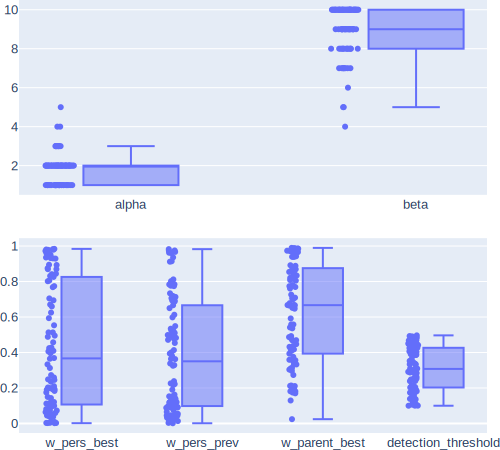
\includegraphics[width=0.85\textwidth]{results/part2/parameter_boxplot_None.svg}
	\caption[Statistical box plot of \gls{hsppbo} parameters]{Statistical box plot of all \gls{hsppbo} parameters (except $H$) over all 90 optimizer runs.}
	\label{fig:parameter_boxplot}
\end{figure}

Starting with the box plot, which is not grouped by any metric, \cref{fig:parameter_boxplot} shows, in addition to the information already described, all 90 values for each parameter as scattered dots next to the box itself. The results for $\alpha$ suggest that it is the most robust parameter of the six, with the median falling together with the upper quartile at 2, and the minimum and lower quartile sharing their value at 1. A value of $\gls{iqr} = 1$ is remarkably low and can only be improved later on in the analysis, when looking at aggregated box plots. The \gls{gbrt} surrogate model seemed to have no problem finding appropriate values for $\alpha$, and since a value of zero was never chosen, a floor effect can be ruled out. The $\beta$ shows a much larger spread around its median of 9 and has a very low fence of 5. However, its \gls{iqr} of 2 suggests that the \gls{hpo} process was mostly consistent in finding values for this parameter. The abrupt end of the upper quartile and the maximum at 10 suggests a ceiling effect (see \cref{chap:choice-param}), which was supposed to be avoided by a sufficiently large value range. Apparently, an upper limit of 10 was not enough for $\beta$. However, since at least 50\% of the values are at or below 9, this effect should not have had a significant influence on the choice of this parameter during \glsdesc{hpo}. 

The three weights, $w_{\text{persbest}}, w_{\text{persprev}}$, and $w_{\text{parentbest}}$, on the other hand, show considerably high dispersion. In particular, the box plot for $w_{\text{persbest}}$ has an $\gls{iqr} = 0.72$, which is almost as large as the possible value range from 0 to 1, with the whiskers reaching these boundaries. Therefore, the median of 0.37 has almost no significance in choosing an optimal parameter based on means alone. This situation improves slightly when looking at the remaining two weights. Although their box plots also span the entire value range, their \gls{iqr} is at about half of the range ($\gls{iqr}_\text{persprev} = 0.57, \gls{iqr}_\text{parentbest} = 0.48$). Therefore, the medians of $w_{\text{persprev}}$ at 0.35 and of $w_{\text{parentbest}}$ at 0.66 can both be considered somewhat robust. However, the fact that all three of these weights are used together in a sum makes any value suggestion an almost random one. Only the absolute parameter configuration range between 0 and 1 and a vague specification of this range for the latter two weights can be confirmed to some extent.

The box plot for the dynamic detection threshold $\theta$ shares its y-axes with the three weights, but only has a possible value range between 0.1 and 0.5. Therefore, its \gls{iqr} is quite large at 0.22 or more than half of its range. The same dispersed behavior can be seen with its whiskers, which reach their minimum and maximum values almost exactly to the third decimal point. Without any kind of grouping applied to the data, no recommendation can be given for the detection threshold and regarding the \gls{hpo} process, this parameter could not be chosen reliably.

\begin{figure}[h]
	\centering
	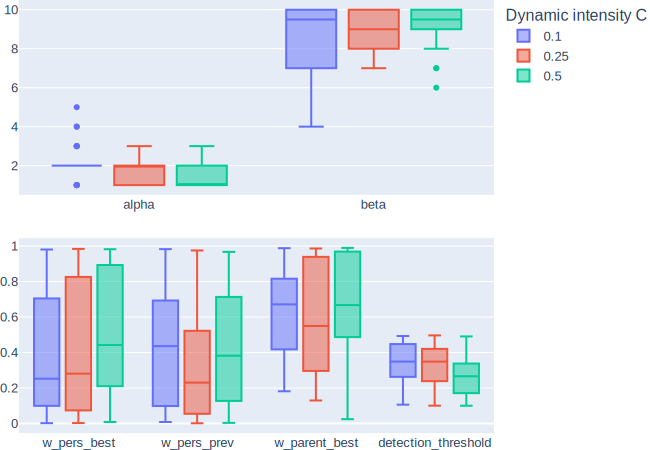
\includegraphics[width=\textwidth]{results/part2/parameter_boxplot_dynamic.svg}
	\caption[Statistical box plot of \gls{hsppbo} parameters compared by dynamic intensity]{Statistical box plot of all \gls{hsppbo} parameters (except $H$) over all 90 optimizer runs and compared by dynamic intensity $C$.}
	\label{fig:parameter_boxplot_dynamic}
\end{figure}

Continuing with the box plots shown in \cref{fig:parameter_boxplot_dynamic}, where the data points are grouped by the three dynamic intensities $C$ tested, an interesting trend emerges for $\alpha$ and $\beta$. For a low dynamic intensity, i.e. very few cities swap places every $T_d = 100$ iterations, an $\alpha$ value of exactly 2 seems to be the ideal choice for the \gls{hpo} process, with an \gls{iqr} of 0 and only four outliers in total. Parameter $\beta$, on the other hand, shows a similarly low dispersion for the highest dynamic of $C = 0.5$. With an $\gls{iqr} = 1$ and a median of 9.5, a strong heuristic influence seems to be beneficial in obtaining good solutions in highly dynamic problems. In the case of $\alpha$, the other two higher dynamics introduce more spread in the choice of values, but always remain in a median range between 1 and 2, with a small dispersion of 1. For $\beta$, the robustness decreases significantly with lower dynamic intensity, reaching a high $\gls{iqr} = 3$ for $C = 0.1$.

As with the ungrouped box plots, the three weights show no sign of robust value behavior. Although small improvements can be observed for certain weights under certain dynamic intensities, e.g., $w_{\text{parentbest}}$ has a comparatively low dispersion of $\gls{iqr} = 0.4$ and a reduced minimum for $C=0.1$, the spread is still far too large to provide any value suggestions under certain dynamic environments. 
Aside from the robustness, the two personal weights, $w_{\text{persbest}}, w_{\text{persprev}}$, have a particularly different median for the lowest dynamic of $C=0.1$, although the medians for the other dynamic intensities are quite similar. This may be due to the fact that, especially in a low dynamic environment the populations for both personal weights become equal after a certain number of \gls{hsppbo} iterations. Therefore, a reset of the personal best population (whether partial or full) still gives the \gls{sce} a copy of that solution through the personal previous solution, which then influences that weight to be more important during \gls{hpo}.

The same statements about robustness can be made for the dynamic threshold $\theta$, where an improvement in the \gls{iqr} of about 0.05, which is 12.5\% of its value range, still does not allow for a sophisticated parameter choice. The only hinted trend might be, contrary to intuition, that lower values of $\theta$, i.e. less \gls{sce} tree swaps necessary to trigger the change handling procedure, benefit solving higher dynamic problem instances ($C=0.5$). However, with a median of 0.27, the upper quartile region still completely overlaps with the other two groups.

\begin{figure}[h]
	\centering
	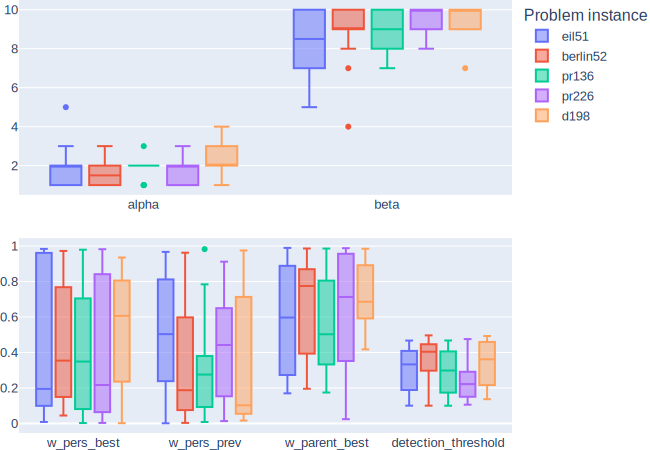
\includegraphics[width=\textwidth]{results/part2/parameter_boxplot_problem.svg}
	\caption[Statistical box plot of \gls{hsppbo} parameters compared by problem instance]{Statistical box plot of all \gls{hsppbo} parameters (except $H$) over all 90 optimizer runs and compared by problem instance.}
	\label{fig:parameter_boxplot_problem}
\end{figure}

\Cref{fig:parameter_boxplot_problem} shows the parameter box plots grouped by the \gls{tsp} problem instance on which they were acquired on. The parameter $\alpha$ shows a low dispersion for \texttt{pr136}, an instance with a moderately clustered structure, and an unusually high dispersion for \texttt{d198}, an instance with highly clustered areas. The other problem instances show similar results as before, and the median for all five instances is still between 1.5 and 2. The same conclusions can be drawn for $\beta$, where the instances \texttt{berlin52, pr226}, and \texttt{d198} show low \glspl{iqr} of 2, while the remaining two instances, especially \texttt{eil51}, show very unreliable values with medians as low as 8.5. 

The three weights show very dispersed distributions, as expected from previous observations, with \texttt{eil51} probably being the most spread out of all values. Only some instances have an improving effect on the robustness, e.g. $w_{\text{persprev}}$ for instance \texttt{pr136} with a low $\gls{iqr} =  0.29$ and a median of 0.28, or $w_{\text{parentbest}}$ for instance \texttt{d198} with $\gls{iqr} =  0.30$ and a median of 0.69. Also, compared to the values from the previous figures, $w_{\text{parentbest}}$ seems to be much more robust across all instances (except \texttt{pr226}), suggesting that this value could be very dependent on the particular problem it is used for.
The detection threshold $\theta$ shows in some instances, i.e. \texttt{berlin52} and \texttt{pr226}, a more robust value selection with \glspl{iqr} around 0.15, which is even better, than the aggregation by dynamic intensity shows. However, these two robust values are very different, with medians of 0.40 and 0.22, respectively, suggesting that dynamic detection may be strongly influenced by the problem instance on which it is used on. This is also seen in the data for the reaction type $H$, which is discussed in the following.
 
\begin{table}[h]
	\centering
	\caption[The distribution of the \gls{hsppbo} reaction type $H$]{The distribution of the \gls{hsppbo} reaction type $H$. Either for all parameter sets or for parameter sets grouped by dynamic intensity $C$ or problem instance, the percentages of these sets using one or the other reaction type are given.}
	\label{tab:reaction-type}
	
	\begin{tabular}{ccS[table-omit-exponent, fixed-exponent = -2, round-precision = 1]S[table-omit-exponent, fixed-exponent = -2, round-precision = 1]}
		\hline
		Comparison & Group & $H_\text{partial}$ [\si{\percent}] & $H_\text{full}$ [\si{\percent}] \\ \hline
		- & - & 0.6666666666666666 & 0.3333333333333333 \\  \hline
		\multirow{3}{*}{Dynamic Intensity} & 0.1 & 0.7666666666666667 & 0.23333333333333334 \\ 
		& 0.25 & 0.5666666666666667 & 0.43333333333333335 \\ 
		& 0.5 & 0.6666666666666666 & 0.3333333333333333 \\ \hline
		\multirow{3}{*}{\shortstack{Dynamic Intensity\\Best 50\% RPD}} & 0.1 & 0.6666666666666666 & 0.3333333333333333 \\ 
		& 0.25 & 0.5333333333333333 & 0.4666666666666667 \\ 
		& 0.5 & 0.6666666666666666 & 0.3333333333333333 \\ \hline
		\multirow{5}{*}{Problem Instance} 
		& eil51 & 0.6111111111111112 & 0.3888888888888889 \\ 
		& berlin52 & 0.7222222222222222 & 0.2777777777777778 \\ 
		& pr136 & 0.7777777777777778 & 0.2222222222222222 \\ 
		& pr226 & 0.8333333333333334 & 0.16666666666666666 \\
		& d198 & 0.3888888888888889 & 0.6111111111111112 \\  \hline
		\multirow{5}{*}{\shortstack{Problem Instance\\Best 50\% RPD}} 
		& eil51 & 0.5555555555555556 & 0.4444444444444444 \\ 
		&  berlin52 & 0.6666666666666666 & 0.3333333333333333 \\ 
		& pr136 & 0.6666666666666666 & 0.3333333333333333 \\ 
		& pr226 & 0.7777777777777778 & 0.2222222222222222 \\ 
		& d198 & 0.4444444444444444 & 0.5555555555555556 \\ \hline
	\end{tabular}
\end{table}

The dynamic reaction mechanism $H$ was chosen to be discussed separately, because a two-valued categorical value is not effectively represented by a box plot. Instead, \cref{tab:reaction-type} shows the distribution across the same comparison groups as used in the box plots. In addition to the two grouped versions, distributions for only those parameter sets that resulted in 50\% or better relative solution qualities ($RPD$) were added to represent what values the best parameter sets use for $H$.

It is immediately evident that the partial reaction $H_\text{partial}$ is most often preferred by the \glsdesc{hpo}, except for some deviations. In the overall (ungrouped) comparison, twice as many parameter sets used this method of dynamic reaction. For the lowest ($C=0.1$) and highest ($C=0.5)$ dynamic intensities, this preference can also be confirmed, while for medium intensity, $H_\text{full}$ is also a viable choice 43.3\% of the time. Except for a slight percentage decrease for $H_\text{partial}$ with $C=0.1$, this behavior does not change for the best 50\% of solutions.
When grouped by \gls{tsp} instance, the only problem that does not favor a partial reset appears to be \texttt{d198}, where 61.1\% of the parameter sets use the $H_\text{full}$ method. Contrary to this observation, the \gls{hpo} process chose the partial reset 83.3\% of the time for \texttt{pr226}, which is the highest bias toward any $H$ method. Looking at the best 50\% of parameter sets, \texttt{eil51} clearly deviates from any preference and has both methods almost at 50\%. The other instances also show a decrease in their bias towards $H_\text{partial}$, except for \texttt{d198}, which now seems to choose the full reset less often for its better solutions.

\subsubsection{Parameter Value Recommendations}
\label{chap:param-recommend}

Based on the previous discussion of parameter robustness, their median values, and possible preferences and trends with respect to certain combinations of dynamic intensity and problem instance, some general recommendations for potentially well-performing parameter sets are given. These suggested value ranges could be used to refine the \gls{hpo} parameter configuration or as guidelines for manual parameter tuning.

Starting with the two most robust recommendations, $\alpha$ and $\beta$, which had the lowest \glspl{iqr} out of all parameter box plots. The median for $\alpha$ was almost always at 2, with boundaries rarely exceeding the interval $[1,2]$. This was also the parameter that was least affected by a change in the problem description, making the choice of $\alpha = 2$ the most robust suggestion. The parameter $\beta$ usually had a median between $[9,10]$ and is slightly influenced by dynamic intensity and problem instances. Since in some combinations $\beta$ was chosen as low as 4, with a lower quartile value of around 7, and considering the ceiling effect, a value range between $[7,12]$ might lead to satisfactory solutions.

The dynamic reaction type $H$ was also most often chosen as $H_\text{partial}$. The influence of different dynamic intensities also seems to be marginal, since only the medium dynamic ($C=0.25$) leads to a change in the distribution, with the highest and lowest tested values still favoring the partial reset. This also holds true for the problem instances, where the results only suggest that certain city placement characteristics - very regular instances like \texttt{eil51} (group 1) or highly clustered instances like \texttt{d198} (group 5) - might have an influence on this choice. Nevertheless, the data indicates that the $H_\text{partial}$ method is the preferred option.

The three weights, $w_{\text{persbest}}, w_{\text{persprev}}$, and $w_{\text{parentbest}}$, are not only agnostic to varying dynamic intensities and problem instances, but their choice also seems to be influenced by some other, possibly random, relationship. Regardless, their median values may still be useful as a symptom of the underlying well-performing parameter sets. The parameter $w_{\text{persbest}}$ has a median between 0.28 and 0.44, and is only influenced by higher dynamics ($C=0.5$) and certain, highly clustered, problem instances (\texttt{d198}). On the other hand, $w_{\text{persprev}}$ seems to be strongly influenced by dynamic intensity and problem instance, resulting in a median between 0.10 and 0.50. And $w_{\text{parentbest}}$, which has the lowest \gls{iqr} of the three, has its median range between 0.50 and 0.78, showing a slight dependence on dynamic intensity and a stronger influence from problem instances. Also, since this range is above the other two weights, it could be implied that the parent-best population might be slightly more significant to the solution construction procedure. These three median ranges can be used as value range suggestions and at least somewhat confirm the \gls{hpo} configuration range between 0 and 1, with no strong floor or ceiling effect present in the data.  

Finally, the detection threshold $\theta$ was slightly influenced by the dynamic intensity, with an interesting preference towards lower values of 0.27 for highly dynamic intensities of $C=0.5$, and was strongly influenced by problem instances. Again, the configured \gls{hpo} value range between 0.1 and 0.5 was confirmed in terms of the lower and upper quartiles never getting too close to these boundaries. However, the high median interval for the problem aggregated statistic of $[0.22, 0.40]$ still spans half of the available range, with the advantage that this suggestion still narrows the range.

In summary, the following parameter range configuration can be seen as a possible refinement to the one given in \cref{chap:choice-param} to reduce the number of objective calls needed to find good parameter sets using \gls{hpo} with \gls{gbrt} for the \gls{hsppbo} metaheuristic, regardless of dynamic intensity or \gls{tsp} problem instance:
\begin{itemize}
	\item $\beta \in \left\lbrace x\in\mathbb{N} | 7 \leq x \leq 12 \right\rbrace$
	\item $w_{\text{persprev}} \in [0.10,0.50]$
	\item $w_{\text{persbest}} \in [0.28,0.44]$
	\item $w_{\text{parentbest}} \in [0.50,0.78]$
	\item $\theta \in [0.22,0.40]$
	\item $H = H_{\text{partial}}$ (not optimized)
	\item $\alpha = 2$ (not optimized) 
	\item $L_\text{pause} = 5$ (not optimized)
\end{itemize}
 In addition, this configuration should further speed up the optimization process and may even increase the quality of the solutions found by reducing the dimensions of the configuration space.

\subsection{Parameter Interaction and Influences}

Besides the analysis of the parameter robustness, another point of interest is the parameter interaction, not only among themselves, but also with respect to certain dynamic intensities.
For this purpose, scatter matrix plots were generated showing every possible combination of two \gls{hsppbo} parameters on the x- and y-axis, respectively, with an optional aggregation over dynamics. Since the resulting matrix would have been antisymmetric, the upper right triangle was omitted to improve readability. The resulting assignment of a parameter to a particular axis, rather than showing the opposite paring as well, does not reflect any real dependence of one parameter on another. As with the previous box plots, the reaction type $H$ was excluded not only for lack of information gain, but also to reduce the size of the matrix and make the figure legible on paper. When analyzing the scatter plots, the ungrouped and dynamic-aggregated figures are used together for each parameter pairing, rather than being discussed one after the other.

\begin{figure}[h]
	\centering
	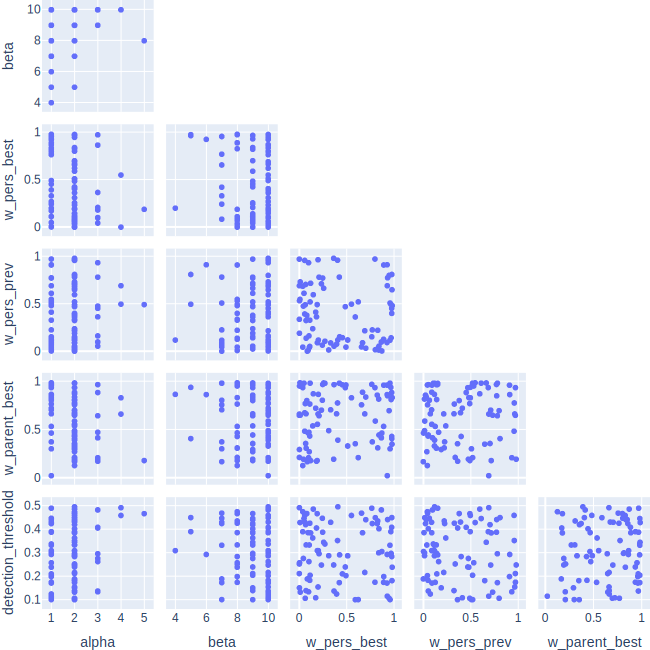
\includegraphics[width=\textwidth]{results/part2/param_scatter_matrix_None.svg}
	\caption[Scatter matrix plot of all \gls{hsppbo} parameters]{Scatter matrix plot of all \gls{hsppbo} parameters (except $H$) over all 90 optimizer runs.}
	\label{fig:parameter_scatter_matrix}
\end{figure}

\begin{figure}[h]
	\centering
	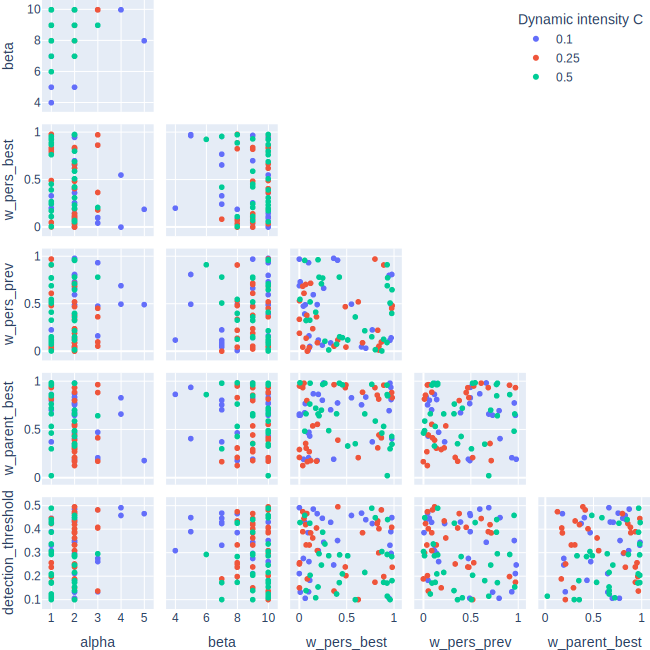
\includegraphics[width=\textwidth]{results/part2/param_scatter_matrix_dynamic.svg}
	\caption[Scatter matrix plot of all \gls{hsppbo} parameters compared by dynamic intensity]{Scatter matrix plot of all \gls{hsppbo} parameters (except $H$) over all 90 optimizer runs and compared by dynamic intensity $C$.}
	\label{fig:parameter_scatter_matrix_dynamic}
\end{figure}

Starting with the ungrouped scatter matrix, \cref{fig:parameter_scatter_matrix}, and looking at the first parameter pairing, with values for $\alpha$ on the x-axis and values for $\beta$ on the y-axis, we can see an interesting distribution towards the upper left corner of the plot. This suggest a correlation, with higher $\beta$ values, between 8 and 10, allowing for higher $\alpha$ values, between 2 and 4. This confirms the relationship between these two parameters for many other metaheuristic parameter tuning procedures as well. However, some parameter sets with high $\beta$ values between 8 and 10, also found small $\alpha$ values of 1 to produce favorable solutions. Furthermore, the region of high values for $\alpha$ and low values for $\beta$ seems to be of little interest for good parameter sets. 

\Cref{fig:parameter_scatter_matrix_dynamic} shows yet another probable correlation due to the influence of different dynamics. In the case of overlapping points, the color of the dynamic intensity was displayed, which is the most common for this parameter combination.
For $\alpha$ and $\beta$, interesting enough, the previously preferred combination of high values of $\beta$ allowing higher values of $\alpha$ most often applies to low dynamic intensities of $C=0.1$, while the opposite correlation, $\beta \in [4,5]$ and $\alpha = 1$, is also used for this dynamic. For the highest dynamic intensity of $C=0.5$ the values for $\alpha$ were not chosen as high with increasing $\beta$, implying that the heuristic influence is relatively more important than the stochastic solution construction for highly dynamic problems.

Continuing down one row, we have $w_{\text{persbest}}$ being paired with $\alpha$ and $\beta$. First, for $\alpha=1$ there is an unusual, but significant gap for the value of $w_{\text{persbest}}$ between 0.5 and 0.75, which increases even further for $\alpha=3$, but inexplicably disappears for $\alpha=2$. Similar gaps in the choice of values can also be found for $\beta = 8$. In the case of the dynamic comparison, no further trend can be found in the scatter plots, except for the value choices already discussed in the previous subsection.

For $w_{\text{persprev}}$, there are only value gaps for $\alpha = 3$ and $\beta = 8$. Especially for the pairing with $\beta$, there is a slight trend towards smaller values for $w_{\text{persprev}}$ for smaller $\beta$ values, with an interesting area for the lowest dynamic intensity of $C=0.1$ and a $\beta = 7$ using unusually low values for $w_{\text{persprev}}$ between 0 and 0.2. The combination of $w_{\text{persprev}}$ and $w_{\text{persbest}}$ shows a significant avoidance of a medium-value area where both parameters are around 0.5, with only four exceptions. Therefore, it is implied that these two parameters are preferred in pairings near the value boundaries, with a small bias towards a low-low-combination. In particular, for a medium dynamic environment of $C=0.25$, lower values for $w_{\text{persprev}}$ below 0.2 are most often used with similarly low values for $w_{\text{persbest}}$.

The parameter $w_{\text{parentbest}}$ shows no clear trend when interacting with $\alpha$ or $\beta$. As with the interaction between the other two weights, the pairing with both $w_{\text{persprev}}$ and $w_{\text{persbest}}$ shows the same avoided mid-area around values of 0.5 for both parameter, although not as pronounced. The bias towards higher values for $w_{\text{parentbest}}$ above 0.2, especially at low dynamic intensities, can also be seen in these scatter plots. Another interesting area to note is present in the pairing with $w_{\text{persprev}}$, where a clear notch in the distribution is visible for $w_{\text{parentbest}} \in [0.8,1]$ and $w_{\text{persprev}} \in [0.2,0.5]$. However, this does not justify an indication of a possible correlation and could just be a random influence. 

Finally, the detection threshold $\theta$ is paired with all other parameters. With $\alpha = 2$, there is a preference for smaller values of $\theta < 0.3$ for high dynamic intensities of $C=0.5$. The opposite can be observed at low dynamics of $C=0.1$ with smaller $\beta \leq 7$ that are being paired with $\theta$ values greater than 0.3. The interaction with any of the three weights does not show any obvious correlation or tendency towards certain areas.

For completeness, \Cref{fig:parameter_scatter_matrix_added} in \cref{chap:figures} also shows the ungrouped version of the scatter plot that includes the dynamic reaction parameter $H$. However, other than avoiding the full reset method ($H_\text{full}$) for low detection threshold $\theta$ values between 0.1 and 0.15, nothing noteworthy is added by this matrix.

In conclusion, only the interaction between $\alpha$ and $\beta$ seems to suggest some kind of correlation between these parameters. In particular, since $\alpha$ is used as an exponent for the sum of the three weights, one might expect some kind of relationship between these parameters. But even when $\alpha$ was plotted in a semi-logarithmic scatter plot over the sum of all three weights (see \cref{fig:alpha_weight_semilog_plot}), no particular distribution became apparent. Therefore, at least for this specific case of \gls{hpo} using \gls{gbrt}, there does not appear to be a direct relationship between these parameters. The same can be said for any other combination of parameters where no zero-order correlation is apparent. However, a higher order correlation across multiple parameters may still be possible and could be further investigated with a different test setup that also samples parameter areas that lead to sub-optimal solutions, i.e., that is not driven by \gls{hpo} goals.


\subsubsection{Partial Dependence}

Although we have already discussed the abundance of strong correlations between parameter pairings, the following partial dependence plots, as described in \cref{chap:an-part2}, take advantage of the predictive capabilities of the final surrogate model generated during \gls{hpo}. Since each of the 90 optimizer runs produced one model, only the model with the best solution quality was used, following the same reasoning as for the selection of the optimal parameter sets described at the beginning.

For each parameter (dimension), 60 points were evaluated across their value ranges, with each point averaged over 250 prediction samples. In the one-dimensional case, shown in the diagonal line plots, this allows for an analysis of the effect of a single dimension on the predicted objective function, i.e., which parameter values most affected the output of the surrogate model. In the two-dimensional case shown below the diagonal, this effect is shown for a combination of two parameters using contour plots. Light colored (yellow) areas represent better solutions (smaller prediction for tour length $L$), while dark colored (blue) areas represent worse solution areas. The black dots represent the observed points during the \gls{hpo}, and the red star in each contour plot marks the best observed parameters. Due to the qualitative nature of these visualizations, and since this is only a strong estimate of what might be really important for the actual \gls{hsppbo} metaheuristic, no explicit quantitative color-map is used, and the $PD$ values on the diagonal one-dimensional plots are to be understood only as relative orientation.

Due to the size of these partial dependence plots, not all 15 possible figures are shown in the following, but only the two most interesting ones, showing the results for the problem instance \texttt{berlin52} and for dynamic intensities $C={0.25,0.5}$, are discussed. However, these two chosen figures are most representative, especially in the context of the analysis from previous subsections, and necessary remarks for the other unused figures will be included if necessary. These other 13 figures are also available in the GitHub repository of this thesis.

\begin{figure}[h!]
	\centering
	\centerline{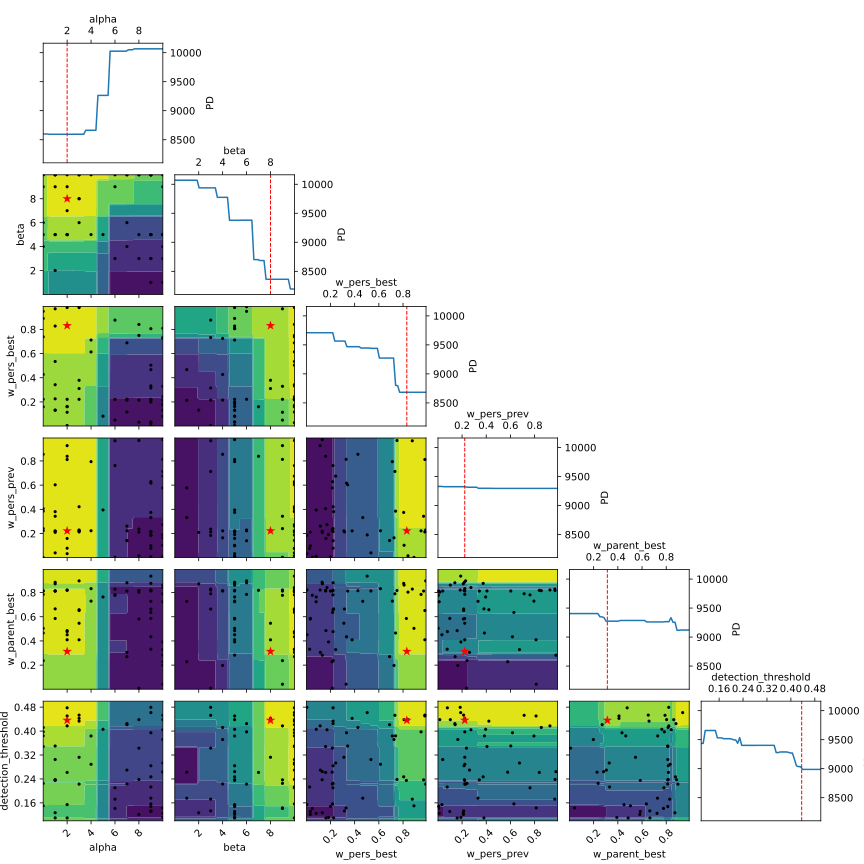
\includegraphics[width=1.2\textwidth]{results/part2/partial_dependence_berlin52_C_0.25_run_4.svg}}
	\caption[Partial dependence plot for \texttt{berlin52} and $C=0.25$]{Partial dependence plot using the surrogate model of the optimizer run with the best parameter set for problem instance \texttt{berlin52} and dynamic intensity $C=0.25$. Better (smaller) solutions are lightly colored, dark areas represent worse solution areas.}
	\label{fig:partial_dependence_berlin52_C_025}
\end{figure}

\Cref{fig:partial_dependence_berlin52_C_025} shows the partial dependence for $C=0.25$. Starting from the diagonal, a low value for $PD$, i.e. a good solution quality, was obtained by the model for $\alpha$ values between 1 and 4, with a steep edge around $\alpha=5$. The solution quality also seems to improve dramatically for higher values of $\beta$, with $\beta \geq 8$ as the optimum. The resulting combination of the two, shown in the contour plot to the left and below these two one-dimensional plots, confirms similar value areas as described previously in \cref{fig:parameter_scatter_matrix}, where the light-colored, good areas are in the upper left corner of the plot, i.e., the high $\beta$, low $\alpha$ value range. The opposite dark blue corner also confirms that this area of high values for $\alpha$ and low values for $\beta$ also leads to predicted bad solutions for the model, which is why this area was never part of a good parameter set. This observation for $\alpha$ and $\beta$ can be made for almost all of the other 14 partial dependence plots, with the only difference that $\alpha$ sometimes has significantly less influence on a good solution, resulting in the contour plot suggesting good solutions for any $\alpha$ value paired with $\beta \geq 8$.

Continuing on the diagonal, high values for $w_{\text{persbest}}$ seem to have a large impact on the solution quality for the predictive model, with $w_{\text{persbest}} > 0.8$ as the optimum. Interestingly, this result differs greatly from previous observations from the statistical box plots grouped by problem instance, where \texttt{berlin52} had a median of 0.35. The contour plots also show clear preferences for high values of $w_{\text{persbest}}$ in combination with high values of $\beta$ and especially with low values of $\alpha$.

On the other hand, the model predicts the same $PD$ regardless of any value of $w_{\text{persprev}}$. This is also evident in the contour plots of the same row, where the light-colored good solution areas are only affected by well-performing $\alpha$ and $\beta$ values, respectively. This is also true for the combination of $w_{\text{persbest}}$, where the avoided area shown in the scatter matrices is also absent.

The parameter $w_{\text{parentbest}}$ has a small influence on the model prediction, with values $ > 0.85$ being most beneficial for a low $PD$. However, this influence does not appear to be sufficient when looking at the contour plots for the first three parameters from the left, where a similarly distinct edge can be seen that is mainly influenced by these more influential parameters. In combination with $w_{\text{persprev}}$, almost no area seems to be of real interest except for a narrow region in the upper right, suggesting that the previously mentioned high values for $w_{\text{parentbest}}$ should be paired with also high values for $w_{\text{persprev}}$.

The detection threshold $\theta$ showed its lowest value for $PD$ at $\theta > 0.44$. This value range is also seen in the contour plots, where the light-colored areas are always above 0.4, except in combination with $\beta$ values close to 10, where lower values for $\theta$ are also possible, suggesting that the higher heuristic influence could compensate for scarcer dynamic detection and thus triggered dynamic reaction mechanisms. 
Furthermore, by looking at the red stars, we can see that the \gls{hpo} process almost always chose a parameter in the areas favored by the surrogate model, except for the pairing of $w_{\text{persprev}}$ and $w_{\text{parentbest}}$, where the predicted best, yellow area in the upper right corner, was never even sampled by the aggregation function.

\begin{figure}[h!]
	\centering
	\centerline{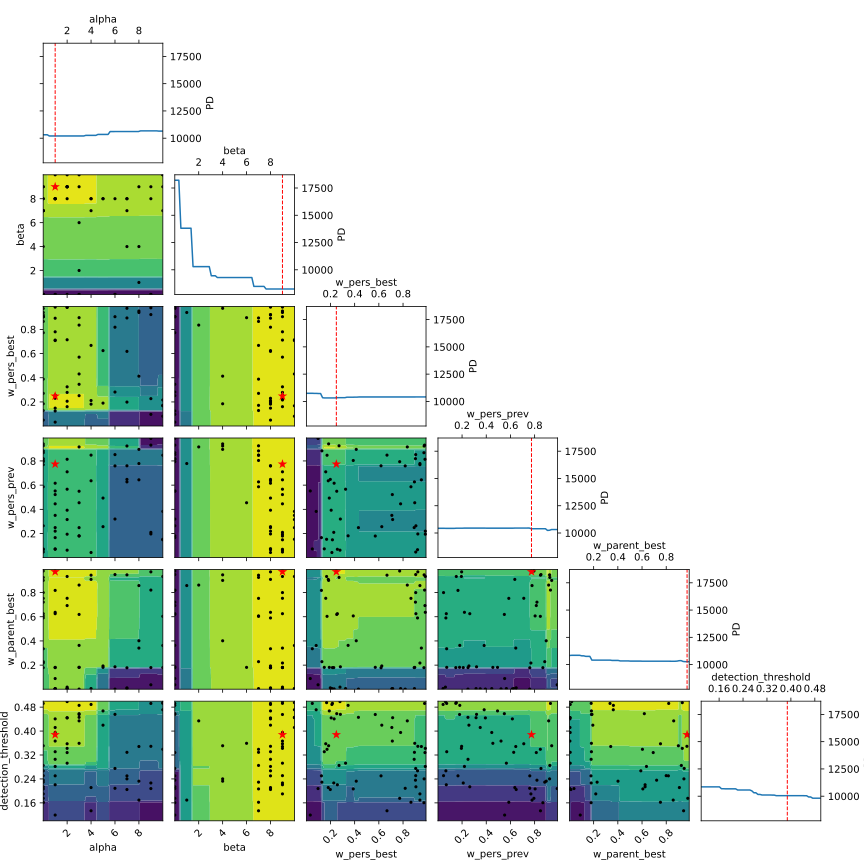
\includegraphics[width=1.2\textwidth]{results/part2/partial_dependence_berlin52_C_0.5_run_4.svg}}
	\caption[Partial dependence plot for \texttt{berlin52} and $C=0.5$]{Partial dependence plot using the surrogate model of the optimizer run with the best parameter set for problem instance \texttt{berlin52} and dynamic intensity $C=0.5$. Better (smaller) solutions are lightly colored, dark areas represent worse solution areas.}
	\label{fig:partial_dependence_berlin52_C_05}
\end{figure}

The second partial dependence plot, \cref{fig:partial_dependence_berlin52_C_05}, shows the results for a higher dynamic intensity of $C=0.5$. 
The same results hold for $\alpha$ and $\beta$, but with the aforementioned lesser influence of smaller $\alpha$ values on $PD$ in the one-dimensional plot. The diagonal plot for $\beta$ also shows a less significant decrease in $PD$ between 4 and 8 than before, instead resembling more of an exponential function. The weight $w_{\text{persbest}}$ is also much less influential for the surrogate model. In fact, the diagonal plots for all three weights show that no particular value in the entire range between 0 and 1 has a significant impact on the prediction of the surrogate model, at least compared to $\beta$. This is also true for the detection threshold $\theta$. The corresponding contour plots for the weights and $\theta$ show similar edges, separating light-colored good solution areas from darker areas, as with $C=0.25$, but with less intense dark-colored spots, suggesting that more areas could result in satisfactory performance. The remaining 13 partial dependence plots show very similar results for the weights and $\theta$.

In addition, compared to the previous, less dynamic representation of the partial dependence, the best observed parameters, indicated by the red stars, are less often in the areas indicated as optimal by the model, suggesting a mismatch between \gls{hpo} and the produced model. In this case, potentially more objective calls or a reduction of the parameter dimension could improve this situation. However, it is quite possible that this mismatch is only produced by the random sampling of the model prediction and is not significantly present in repeated predictions with a different random initialization.

Concluding, we can confirm some relationships between parameters, especially that of $\alpha$ and $\beta$. However, even by using the trained model for its predictive capabilities, we did not gain any further insight into possible direct correlations between parameters. Nevertheless, the importance of certain parameters for the surrogate model is an interesting addition to this analysis.

\subsection{Parameter Importance}
\label{chap:param-importance}

In the previous subsection, regarding the partial dependence plots, we already discussed the influence of the parameters on the surrogate model and its prediction of solution quality. This was achieved by explicitly sampling the parameter search space using the surrogate model. For some simpler \gls{ml} models, mostly decision tree-based, the feature, or in this case the parameter importance, can be  extracted directly from the structure of the model. The previously required intermediate sampling is now replaced by analyzing the structure of the regression trees of the \gls{gbrt} surrogate model used for the experiments. The resulting relative parameter importance, or so-called \glsfirst{mdi}, as explained in \cref{chap:an-part2}, expresses how important a particular parameter is for the prediction of the underlying model. For example, for a simple linear regression, $y = a_0  \cdot x_1 + a_1 \cdot x_1 + ... + a_n \cdot x_n$, the values for $a_i$ would indicate the relative importance for their corresponding parameter $x_i$. 

As mentioned earlier in the experimental setup chapter, the procedure for calculating the \gls{mdi} has some limitations. It has a bias towards parameters with high cardinality and therefore tends to underestimate the importance of parameters such as $H$, which has only two values. Furthermore, it can only reflect the importance resulting from the 60 objective calls during the optimizer run, i.e., it is not a statement about the importance of the entire parameter search space and, as such, of the \gls{hsppbo}. Nevertheless, the \gls{mdi} is still an indicator of what the model considered important enough to base its predictions on, which then guides the successful search for well-performing parameter sets. 

\begin{table}[h]
	\centering
	\caption[Relative parameter importance over all 90 optimizer runs]{The relative parameter importance (\gls{mdi}) computed via the surrogate model over all 90 optimizer runs with the standard error. }
	\label{tab:parameter_importance}
	\begin{tabular}{cccc}
		\hline
		$\beta$ & $\alpha$ & $w_{\text{parentbest}}$ & $\theta$ \\ \hline
		  \num{0.3026887387214929} $\pm$ \num{0.0068271325972591185} & 
		  \num{0.18503797670261257} $\pm$ \num{0.005773445553779512} & 
		  \num{0.13219322556428054} $\pm$ \num{0.0048906270152243485} & 
		  \num{0.1316600435540604} $\pm$ \num{0.005210027993794393} \\ \hline
	\end{tabular}
	\bigskip\\
	\begin{tabular}{ccc}
		\hline
		$w_{\text{persprev}}$ & $w_{\text{persbest}}$ & $H$ \\ \hline
		\num{0.11494569405569222} $\pm$ \num{0.004096682063210092} & 
		\num{0.10821824956197788} $\pm$ \num{0.003648963763332609} & 
		\num{0.025256071839883553} $\pm$ \num{0.0023011990335138335} \\ \hline
	\end{tabular}
\end{table}


\cref{tab:parameter_importance} shows the averaged \gls{mdi} for all \gls{hsppbo} parameters with their standard errors over all 90 optimizer runs. The table is also ordered from the most highest value (left) to the lowest value (right), and all values sum to 1. The importance of the parameter $\beta$ is by far the highest at 0.303, indicating that about a third of each model-prediction is explained by this value. The standard error is also the highest by comparison, but still very low and far away from the margin of error for the second most important parameter, $\alpha$, at 0.185. This difference of more than 10\% between the first and second most important parameters suggests that although this \gls{mdi} metric is biased, $\beta$ is definitely an important parameter for the \gls{hsppbo} metaheuristic. Including the importance of $\alpha$ may also explain why only these two parameters were the most robust and consequently allowed for a reasonably meaningful value suggestion.

The next most important parameters are $w_{\text{parentbest}}$ and $\theta$, both with $\gls{mdi} = 0.132$, also with very low standard errors when averaged over all optimizer runs. In particular, $w_{\text{parentbest}}$ showed a slightly more robust behavior in the box plots and also had a higher median than the other two weights, thus implying more importance to the solution creation process. Therefore, it seems reasonable that $w_{\text{parentbest}}$ has a higher \gls{mdi} than the other weights.

This is followed by $w_{\text{persprev}}$ at $\gls{mdi} = 0.115$ and $w_{\text{persbest}}$ at $\gls{mdi} = 0.108$, both of which are very close to the previous two parameters, with at most 3\% less importance. Their standard errors are also very small, at around 3.5\% relative to their values. The least important parameter, as already indicated by the bias, is the dynamic reaction type $H$. With only $\gls{mdi} = 0.025$, it is four times less important than the next most important parameter $w_{\text{persbest}}$ and 12 times less important than the most relevant parameter $\beta$.

\begin{figure}[h!]
	\centering
	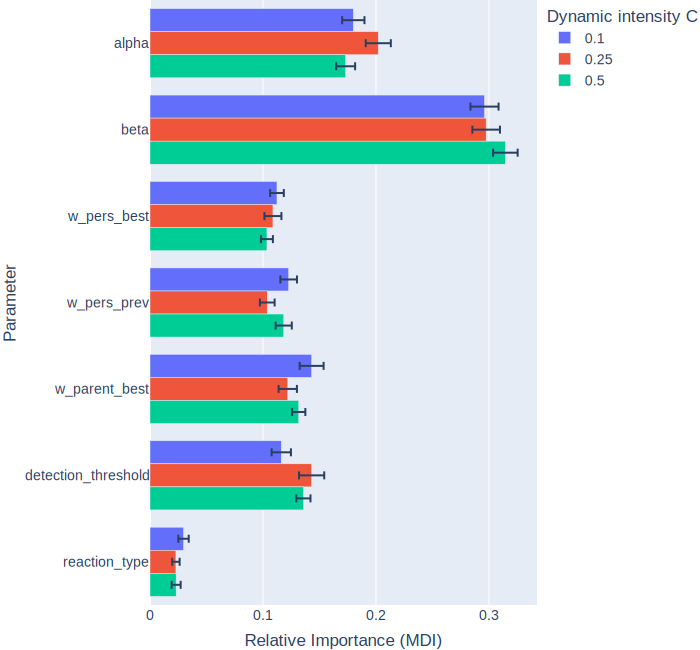
\includegraphics[width=1\textwidth]{results/part2/parameter_importance_bar_dynamic.svg}
	\caption[Bar chart of the parameter importance compared by dynamic intensity]{Bar plot of the parameter importance (\gls{mdi}) computed via the surrogate model over all 90 optimizer runs and compared by dynamic intensity $C$.}
	\label{fig:parameter_importance_bar_dynamic}
\end{figure}

The order of parameter importance does not change when the optimizer runs are grouped by their respective dynamic intensities $C$, as shown by the bar plot in \cref{fig:parameter_importance_bar_dynamic}. Here, the values are also discussed qualitatively for comparison, rather than giving the absolute \gls{mdi} values as before. Most of the differences in \gls{mdi} are within the margin of error, represented by the black whiskers at the right end of each bar. Only an increase in the importance of $\alpha$ and a slight decrease of $w_{\text{persprev}}$ and $w_{\text{parentbest}}$ are noticeable for medium dynamic intensities ($C=0.25$) compared to the other dynamics. Also, the detection threshold becomes slightly more important as the dynamic intensity increases, which could be expected from an increasingly changing problem environment, where improved change detection leads to better solutions. However, all these results are very close to the error margins of their groups and, as already mentioned, do not significantly change their relative importance compared to the values discussed in the previous table. 

\begin{figure}[h!]
	\centering
	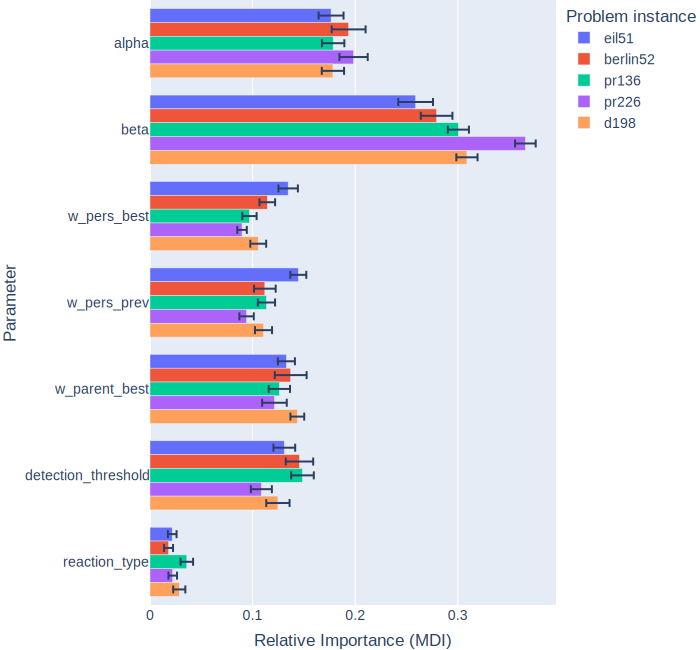
\includegraphics[width=1\textwidth]{results/part2/parameter_importance_bar_problem.svg}
	\caption[Bar plot of the parameter importance compared by problem instance]{Bar plot of the parameter importance (\gls{mdi}) computed via the surrogate model over all 90 optimizer runs and compared by problem instance.}
	\label{fig:parameter_importance_bar_problem}
\end{figure}

Similar findings can be made when grouping across problem instances, where the order parameter of parameter importance remains mostly the same. \Cref{fig:parameter_importance_bar_problem} shows only a few problem instances that change the importance for certain parameters. In particular, the highly clustered instance \texttt{pr226} has an importance of $\beta$ of over 0.35, more than any other instance, with a relatively low standard error. This instance also has $\alpha$ at about the same importance as the overall average, but the weights and detection threshold $\theta$ at even lower importance. In contrast, the very small and semi-regular instance \texttt{eil51} has the lowest importance out of all for $\beta$ and the highest \glspl{mdi} for the parameters $w_{\text{persbest}}$ and $w_{\text{persprev}}$, therefore suggesting an increasing relevance of the personal \gls{sce} populations for the solution creation process. In addition, instance \texttt{pr136} evaluated the reaction type $H$ as more important than any other problem instance. 

In summary, $\beta$ is undoubtedly the most important parameter for the surrogate model in every possible problem scenario, followed by $\alpha$ with about 10\% less relative importance. The three weights and the detection threshold $\theta$ are evaluated with varying importance depending on a certain dynamic intensity and problem instance, so that the importance gap to $\alpha$ is even smaller under some conditions. Finally, the reaction type appears to be the least important parameter, although this statement may be significantly invalidated by the cardinality bias of the \gls{mdi} method. 


\section{Part III - Evaluating the Parameter Sets}

The third part of the evaluation is based on the experimentation data of all ten \gls{tsp} instances, small and large, with all three dynamic intensities $C=\{0.1,0.25,0.5\}$, and each combination of instance and intensity was repeated $r_\text{exp} = 20$ using their specific optimal parameter set acquired by \gls{hpo}. As explained, all the parameters that have been acquired from smaller instances were used for the larger instance in the same structural group (see \cref{tab:best-parameters}). In addition to the \gls{hpo} parameter sets, a generally well-performing reference set based on the results of the original \gls{hsppbo} paper \cite{kupfer2021hierarchical} was used. In visualizations and comparisons, this is denoted as \enquote{Ref}. In contrast to the \gls{hpo} experiments, the parameter set for these reference experiments was the same for all combinations of instance and dynamics.

Furthermore, all graph and table data were computed by averaging the 20 repeated experimentation runs for each instance and dynamic intensity, and for aggregated or grouped data, they were also averaged across different dynamic intensities and/or \gls{tsp} instances. However, this is be mentioned where relevant. Since only \textit{TSPLIB} instances were used, the $RPD$, i.e. the relative difference to the optimal solution, was used to compare the solution quality, as in the first part of the results chapter. Also, as mentioned in \cref{chap:testing}, dynamic events start at iteration 2000 and occur at every next 100th iteration up until the last iteration at 2599. The time between each dynamic events is referred to as dynamic interval.

\subsection{Solution Quality}

After the first two result parts answered the two main research questions, we proceed to the fundamental, underlying question of whether or not these \gls{hpo} parameter sets produce satisfactory results at all. Therefore, the solution quality in the form of the previously used $RPD$ is shown over the course of the dynamic runtime, starting at iteration 1950, just before the first dynamic change is triggered at iteration 2000, and continuing until iteration 2399, omitting the last two dynamic events since they do not add any relevant data. 


\begin{figure}[h]
	\centering
	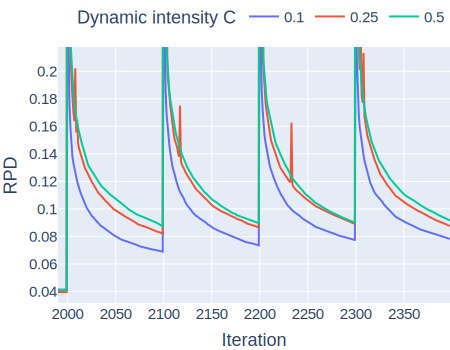
\includegraphics[width=0.7\textwidth]{results/part3/run_plot_cmp_dynamic_aggr_None_y_best_solution_1_to_30_HPO.svg}
	\caption[Line plots showing the $RPD$ over the dynamic iterations for all three dynamic intensities $C$]{Line plots showing the relative solution quality $RPD$ over the first 400 dynamic iterations (starting just before iteration 2000) for all three dynamic intensities $C$ averaged over all instances that used the \gls{hpo} parameter sets.}
	\label{fig:run_plot_cmp_dynamic_HPO}
\end{figure}

\Cref{fig:run_plot_cmp_dynamic_HPO} shows one of these run plots with different lines for each dynamic intensity $C$ and averaged over all \gls{tsp} instances. The first impressive aspect to note is that the solution quality just before the first dynamic event at iteration 2000 is exceptionally good for all dynamic intensities around $RPD=4\%$. Although the solution quality of the first 2000 iterations, representing the static \gls{tsp} problem, was only weighted with $1/7$, compared to the other six solution qualities taken just before the next dynamic event, the influence must have been sufficient for the \gls{hpo} process to produce good results here as well. 

Continuing to the first dynamic event at iteration 2000, there is an expected huge spike in solution quality for all three intensities, which continues along the y-axis up to $RPD=3$ and was truncated to increase the differentiation of the lines between the dynamic events. Interestingly, the medium dynamic intensity $C=0.25$ reached a higher value of $RPD=3$, while the solution quality for the higher dynamic $C=0.5$ did not spike as high to only $RPD=0.7$. This is mainly because the majority of parameter sets at $C=0.25$ used the full reset ($H_\text{full}$) as the change handling procedure, which resulted in significantly worse solution quality immediately after the change was detected, rather than the partial reset, where better performing solutions were still stored in the \gls{sce} tree. At iteration 2008 there is another spike, indicating a delayed execution of the change handling procedure, which can also be observed at different iterations in between each following dynamic interval. These spikes are also due to some specific instances that will be further analyzed at a later time. 

After these first 10 iterations following the dynamic event we observe a rapid increase in solution quality up to iteration 2099, with the parameter sets produced for the least dynamic problems $C=0.1$ clearly leading in $RPD$ value, achieving a solution only about 3\% worse than the static one. The $RPD$ values just before the next three dynamic events at 2200, 2300, and 2400 also show leading performance, although not as good as in this first interval. The solution qualities for the other two dynamic intensities also managed to improve to $RPD_{C=0.25}=0.8$ and $RPD_{C=0.5}=0.9$ just before the next dynamic event, which is also the case for the next three dynamic intervals. 

\begin{figure}[h]
	\centering
	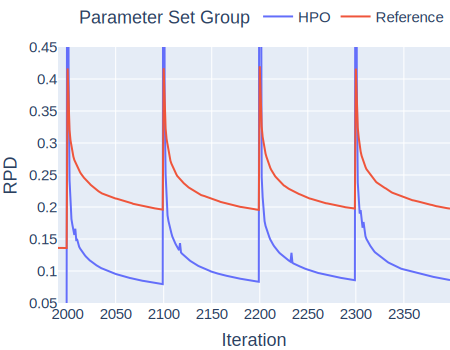
\includegraphics[width=0.65\textwidth]{results/part3/run_plot_cmp_folder_aggr_None_y_best_solution_1_to_30_HPO.svg}
	\caption[Line plots showing the relative solution quality $RPD$ over dynamic iterations for both parameter set groups averaged over dynamic intensities $C$ all \gls{tsp} instances.]{Line plots showing the relative solution quality $RPD$ over the first 400 dynamic iterations (starting just before iteration 2000) for both parameter set groups, \gls{hpo} and the reference set, averaged over all three dynamic intensities $C$ all ten \gls{tsp} instances.}
	\label{fig:run_plot_cmp_folder}
\end{figure}

To put these solution quality values into perspective, \cref{fig:run_plot_cmp_folder} shows the results for the reference parameter set in the same graph as the \gls{hpo} results, averaged over all dynamic intensities and \gls{tsp} instances. Although the reference set also produces acceptable results, the parameters obtained by \gls{hpo} clearly outperform them at every point in the dynamic runtime. Not only is the static solution more than three times better up to iteration 2000 than the reference parameter set ($RPD_\text{HPO} = 0.4$ vs. $RPD_\text{Ref}=0.14)$), the solutions obtained during each dynamic interval, just before the next dynamic event, are also significantly better with more than two times lower $RPD$ values of 0.08 compared to $RPD_\text{Ref}=0.2$. However, the reference parameter set appears to have no noticeable false detections of dynamic change in its dynamic intervals and also spikes to much lower $RPD$ values of just over 0.4.

When viewed separately for each dynamic intensity, as shown in \cref{fig:run_plot_cmp_folder_aggr_dynamic_HPO}, the impression does not change much. Just before each dynamic event, the reference parameter set consistently produced almost the same solution quality of $RPD_\text{Ref}=0.2$, while the \gls{hpo} parameter sets produced better results for lower dynamic intensities of $C=0.1$, as discussed above.

\begin{figure}[h]
	\centering
	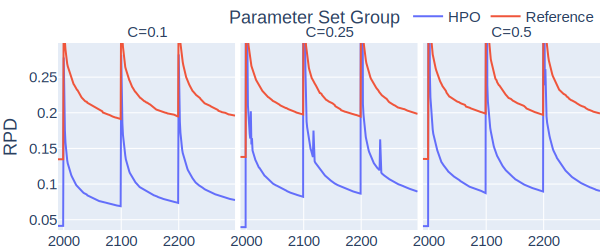
\includegraphics[width=0.85\textwidth]{results/part3/run_plot_cmp_folder_aggr_dynamic_y_best_solution_1_to_30_HPO.svg}
	\caption[Line plots showing the relative solution quality $RPD$ over dynamic iterations for both parameter set groups for each dynamic intensity$C$, averaged over \gls{tsp} instances]{Line plots showing the relative solution quality $RPD$ over the first 300 dynamic iterations (starting just before iteration 2000) for both parameter set groups, \gls{hpo} and the reference set, with a plot for each dynamic intensity$C$, averaged over all ten \gls{tsp} instances.}
	\label{fig:run_plot_cmp_folder_aggr_dynamic_HPO}
\end{figure}

\subsubsection{Problem Instance Generalization}
Next, we want to evaluate the problem classification and the proposed generalization of parameter sets obtained from smaller problem instances to larger instances of the same structural group. For this purpose, \cref{fig:run_plot_cmp_dynamic_aggr_problem_HPO} shows the run plots for each individual \gls{tsp} instance and each dynamic intensity $C$. The instance names are at the top of each plot and they are ordered in the same way as before in \cref{fig:cluster-groups}, so that the smaller instances are in the left column and the larger instances are in the right column, with each row corresponding to the predefined structural groups. Thus, each row of plots uses the same set of parameters when comparing dynamics.

\begin{figure}[p]
	\centering
	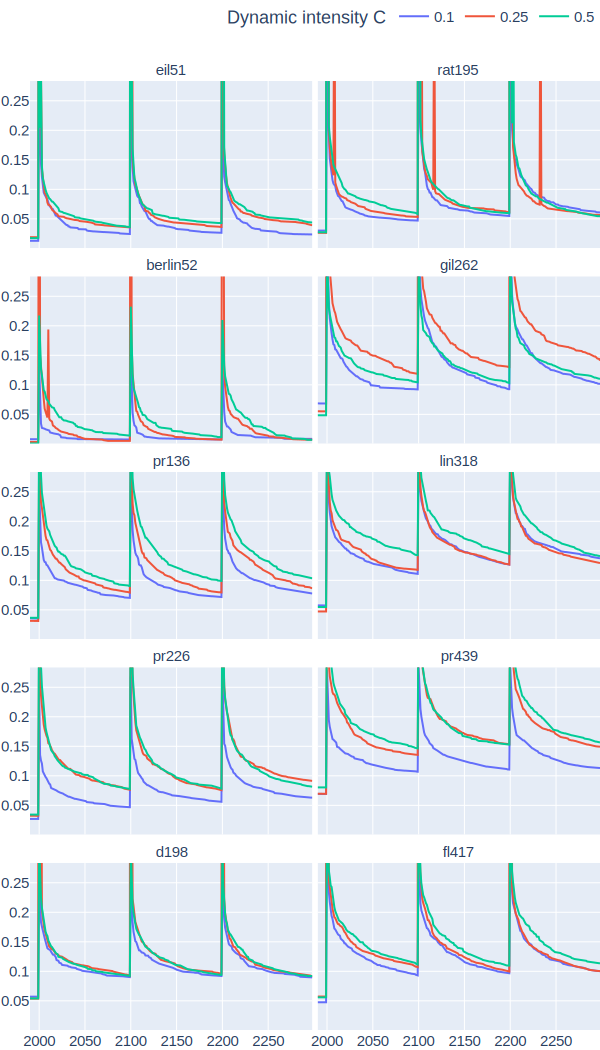
\includegraphics[width=0.725\textwidth]{results/part3/run_plot_cmp_dynamic_aggr_problem_y_best_solution_1_to_30_HPO.svg}
	\caption[Line plots showing the relative solution quality $RPD$ over dynamic iterations for all dynamic intensities $C$ and all \gls{tsp} instances for the \gls{hpo} experiments.]{Line plots showing the relative solution quality $RPD$ over the first 300 dynamic iterations (starting just before iteration 2000) for all three dynamic intensities $C$ and all ten \gls{tsp} instances for the \gls{hpo} experiments. The smaller instances are in the left column and the larger instances are in the right column. Each row corresponds to the predefined structural groups (see \cref{fig:cluster-groups}).}
	\label{fig:run_plot_cmp_dynamic_aggr_problem_HPO}
\end{figure}

The first row shows instances with random to nearly regular distribution. Although \texttt{rat195} has a dimension almost four times larger than \texttt{eil51}, the solution qualities for the static problem and the following dynamic intervals are very similar. With only a few percent worse $RPD$ values for \texttt{rat195} the overall performance just before the end of each dynamic interval is very satisfactory at around $RPD=0.05 \pm 0.01$. Furthermore, the static performance for \texttt{eil51} shows that it was almost perfectly solved for all three dynamic intensities at $RPD_{C=0.1}=0.01$ and $RPD_{C=0.25,0.5}=0.02$, which is even more interesting considering the use of very different parameters for each dynamic intensity. The larger pendant \texttt{rat195} also got very good static performance at around $RPD=0.025$, but has some significant cases of false dynamic detection, even resulting in spikes five iterations ($L_\text{pause} = 5$) after the dynamic event. 
Although both instances used the same parameter sets for $C=0.25$, the higher problem complexity resulted in an increase in \gls{sce} tree swaps many iterations after the dynamic event occurred, which then resulted in a large increases in $RPD$ because $H_\text{full}$ was used as the change handling procedure. 
The differences between the dynamic intensities are very small for both instances, which could be explained by the regular distribution of city nodes and therefore easier solution adaptation process after the problem change.

The second row contains \gls{tsp} instances with smaller, slightly clustered areas with an otherwise random structure. However, the two instances produced very different solution qualities. The \gls{hsppbo} algorithm almost always found the optimal solution in the static part for the smaller instance, \texttt{berlin52}, while the $RPD$ for \texttt{gil262} is only about 5\% just before the dynamic event at iteration 2000. Also, the parameter set used for the low dynamic intensity of $C=0.1$ produced a worse static solution quality than with the other two higher dynamic intensities. Looking at the parameter set in \cref{tab:best-parameters}, this could be explained by the use of the highest value for $\alpha$ across all parameter sets of  $\alpha = 3$, paired with the lowest $w_\text{parentbest}$ value of $w_\text{parentbest} = 0.196$. This could be due to the fact that \texttt{berlin52} has only one fifth of the city nodes of \texttt{gil262}, making it easier to find a good static solution, and the positive influence of these parameters on the dynamic performance. Another interesting observation for \texttt{gil262} is the worse dynamic performance of the parameter set for $C=0.25$ compared to $C=0.5$, although the results for \texttt{berlin52} do not show this behavior. Again, by looking at the parameters used, we can see that for $C=0.25$ a full reset of the \gls{sce} tree ($H_\text{full}$) was used with a very high dynamic detection threshold of $\theta=0.436$, thus making the algorithm less sensitive to dynamic changes in the problem instance. The instance \texttt{eil51} also used a similarly high $\theta = 0.46$ with $H_\text{full}$, but for a the high dynamic intensity of $C=0.5$, which produced better results because the dynamic detection threshold was likely reached more often.

The third row shows more consistent results when comparing the smaller instance, \texttt{pr136}, and the larger instance, \texttt{lin318}. These problems are artificially structured with certain patterns of medium clustered regions, with small distinct holes in the city distribution. The corresponding parameter sets use $\alpha = 2$, low $w_\text{persbest}$, and $H_\text{partial}$ for all three dynamic intensities. This resulted in good static performance just before the first dynamic event in iteration 1999, with $RPD$ values of just under 5\% for \texttt{pr136} and around 5\% for \texttt{lin318}.  The following first dynamic event shows very low spikes in $RPD$ with the highest value being 4\% for $C=0.5$. The increase in solution quality (and the decrease of the curve) seems to be less significant than for \texttt{berlin52} or the first row, and the $RPD$ values just before the next dynamic event do not come close to the static performance, especially for $C=0.5$ where the metaheuristic only obtained a solution of $RPD=0.1$ for \texttt{pr136} and $RPD=0.15$ for \texttt{lin318}, which is one of the worst results for any problem instance. The parameter sets for the two lower dynamic intensities can only marginally improve the $RPD$ values between dynamic intervals. The artificial pattern of city placement appears to make it more difficult to find good solutions after a dynamic change in a short amount of time.

The fourth row shows \gls{tsp} instances with few highly clustered areas, \texttt{pr226} and \texttt{pr439}, which produce a run curve very similar to the previous row. Interestingly, both structural groups share the same value range for the regularity index, which may explain their similar solution quality convergence behavior. They also show similarities in static performance, with \texttt{pr439} having a slightly worse solution quality, and the larger instance \texttt{pr439}, again showing one of the worst dynamic interval performances, only reaching $RPD_{C=0.25,0.5}=0.15$. However, the solution quality for the lowest dynamic $C=0.1$ is much lower for both small and large instances, with differences of up to 5\% in $RPD$, but only in dynamic situations. This suggests that the parameters seem to be highly tuned to perform well for small changes in the problem. Notable values in this set are very low $w_\text{persbest} = 0.112$ and $w_\text{persprev} = 0.051$, comparatively higher  $w_\text{parentbest} = 0.436$, and a low detection threshold of $\theta = 0.183$. Especially the last parameter could have a big impact on the good dynamic performance. However, other instances, such as \texttt{d198}, with a similar $\theta$ value at $C=0.1$ do not show the same good performance. This suggests that the structural characteristics of both problem instances may have had an influence.

The fifth and last row, with instances \texttt{d198} and \texttt{fl417}, represent a dispersed city placement, with highly clustered areas with few or no city nodes in between. The regularity index here is different from the previous two rows (groups). The convergence behavior between dynamic intervals is now more similar to the first row, with a rapid increase in solution quality in the first few iterations after the dynamic event, followed by a stagnation period up until the next dynamic event. Also, the difference between smaller and larger instance is the smallest out of all structural groups, with a gap of only 1-2\% for $C=0.5$. Interestingly, the static performance of the larger instance, \texttt{fl417}, is better than that of the smaller instance, \texttt{d198}, for $C=0.1$, which is also true for the first dynamic interval.

Compared to the same plots for the reference parameter set, shown in the \cref{chap:figures}, \cref{fig:run_plot_cmp_dynamic_aggr_problem_ref}, we can immediately confirm the conclusion from the aggregated plot above. The \gls{hpo} clearly outperforms the reference parameter set, with some instances showing significantly worse solution quality between dynamic events with $RPD$ values over 25\%. Also, the difference between dynamic intensities is not nearly as significant as for the \gls{hpo} parameters, suggesting that the tuning process specific to each dynamic intensity also seems to improve performance.

In summary, all ten \gls{tsp} instances show their own specific solution quality behavior and response to dynamic changes. Although a similar convergence behavior can be found within each structural group, which is also true for the plots for the reference parameter set, the data is not sufficient to suggest a clear relationship to the city placement characteristic. However, the generalization assumption can be confirmed to some extent, since all parameter sets for smaller instances also produced very good results for their larger counterparts. For a more profound evaluation of this aspect, a cross-validation of these parameter sets over different \gls{tsp} instances and dynamic intensities would have been necessary, but would have increased the number of experiments by a factor of 8.5. 

\subsection{Detection of Dynamic Changes}

A very important aspect of the \gls{hsppbo} metaheuristic is its ability to detect changes in the problem it solves and, in response, trigger a change handling procedure to respond optimally. Its performance in this regard depends solely on the dynamic detection threshold $\theta$ and its response mechanism on the $H$ mechanism, $H_\text{full}$ or $H_\text{partial}$. Without any prior knowledge of the way the \gls{hpo} method chooses these parameters, one would assume that, since the main goal is to obtain good solutions in dynamic environments, the correct detection of these changes is of high importance to the algorithm and thus to the \gls{hpo} method.
However, we have already discussed the minor importance of these two dynamic-relevant parameters in the previous results section (see \cref{chap:param-importance}).

Since the results in this respect deviate very strongly from this assumption, the general conclusion should already be anticipated.
With a few exceptions, related to specific combinations of instances and dynamics, and thus individual parameter sets, the correct detection of dynamic changes in the problem does not seem to have a particularly large effect on the solution quality of the \gls{hsppbo} algorithm when using \gls{hpo} parameter sets. More surprisingly, the reference parameter set outperforms the \gls{hpo} parameter sets in every discipline in terms of dynamic detection. This puts into perspective the exceptionally good solution quality performance of the \gls{hpo} parameter sets discussed before and raises the question of how relevant the correct detection of dynamic changes really is for good solutions to the \gls{dtsp}. To support these statements, the following graphs and tables provide performance metrics for many aspects of the dynamic detection behavior. 

First, the number of swaps, i.e., the changes within the \gls{sce} tree that eventually exceed the dynamic detection threshold $\theta$, is plotted over the first three dynamic intervals, similar to the solution quality plots from above. \Cref{fig:run_plot_cmp_dynamic_swaps} shows the results averaged over all ten \gls{tsp} instances, but separated by dynamic intensity $C$, represented by a line for each value. The left line plot shows the \gls{hpo} parameter sets, the right plot shows the reference parameter set. An additional dashed line was drawn for the reference parameter set, indicating the detection threshold $\theta = 0.25$, which results in $0.25 \cdot |A| = 3.25$ swaps required to trigger the change handling procedure. A similar line cannot be drawn for the \gls{hpo} plot because every \gls{tsp} instance uses its own $\theta$ value. A later plot, separated by problem instance, will show more details.

\begin{figure}[H]
	\centering
	\begin{subfigure}{0.515\textwidth}
		\centering
		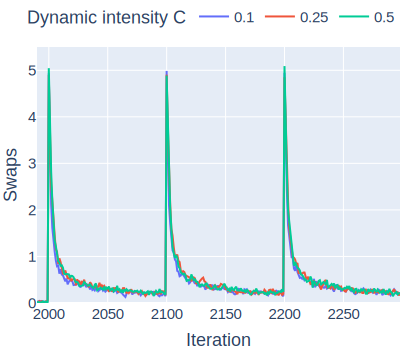
\includegraphics[width=\textwidth]{results/part3/run_plot_cmp_dynamic_aggr_None_y_swaps_1_to_30_HPO.svg}
		\caption{HPO}
		\label{fig:run_plot_cmp_dynamic_swaps_HPO}
	\end{subfigure}
	\begin{subfigure}{0.472\textwidth}
		\centering
		\raisebox{1.5pt}{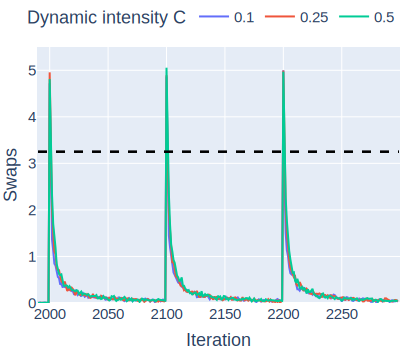
\includegraphics[width=\textwidth]{results/part3/run_plot_cmp_dynamic_aggr_None_y_swaps_1_to_30_Reference.svg}}
		\caption{Reference}
		\label{fig:run_plot_cmp_dynamic_swaps_Reference.svg}
	\end{subfigure}
	\caption[Line plots showing the swaps within the \gls{sce} tree over dynamic iterations for both parameter set groups showing all three dynamic intensities $C$, and averaged over \gls{tsp} instances.]{Line plots showing the relative solution quality swaps within the \gls{sce} tree over the first 300 dynamic iterations (starting just before iteration 2000) with a plot for each parameter set group, \gls{hpo} and the reference set, each showing all three dynamic intensities $C$, and averaged over all ten \gls{tsp} instances.}
	\label{fig:run_plot_cmp_dynamic_swaps}
\end{figure}

The first thing that is immediately noticeable is the similar number of swaps for both parameter groups, with an average of 5 swaps right at the dynamic event for all three dynamic intensities. This makes sense when considering the three levels of the \gls{sce} tree, where the first two levels are very likely to lose their high position when using the partial reset strategy $H_\text{partial}$, resulting in 4 swaps. However, the \gls{hsppbo} algorithm using the reference parameter set has its threshold at a reasonable level, which allows the dynamic response mechanism $H$ to be almost always correctly triggered immediately after the dynamic event. This partial reset allows the algorithm to find new, good solutions, which greatly reduces the number of swaps around 25 iterations after the dynamic event. Eventually, after the 50th iteration in each dynamic interval, the amount of swaps has been reduced to about $0.10 \pm 0.05$ for all the dynamic intensities. Compared to the \gls{hsppbo} results, the amount of swaps after this 50th iteration after each dynamic event is much higher at $0.30 \pm 0.1$, indicating that even long after the dynamic event has occurred, the algorithm is still finding better solutions than its direct parent node at about every third iteration. This suggests that either, the change handling procedure was not triggered, allowing old, possibly bad, solutions to influence the search for a longer time, or that the particular combination of parameters just performed enough exploratory behavior to still find increasingly better solutions at a later time. While the latter theory can be dismissed by looking at the almost identical convergence behavior of the solution quality comparison in \cref{fig:run_plot_cmp_folder}, the former theory is discussed later.

\begin{figure}[p]
	\centering
	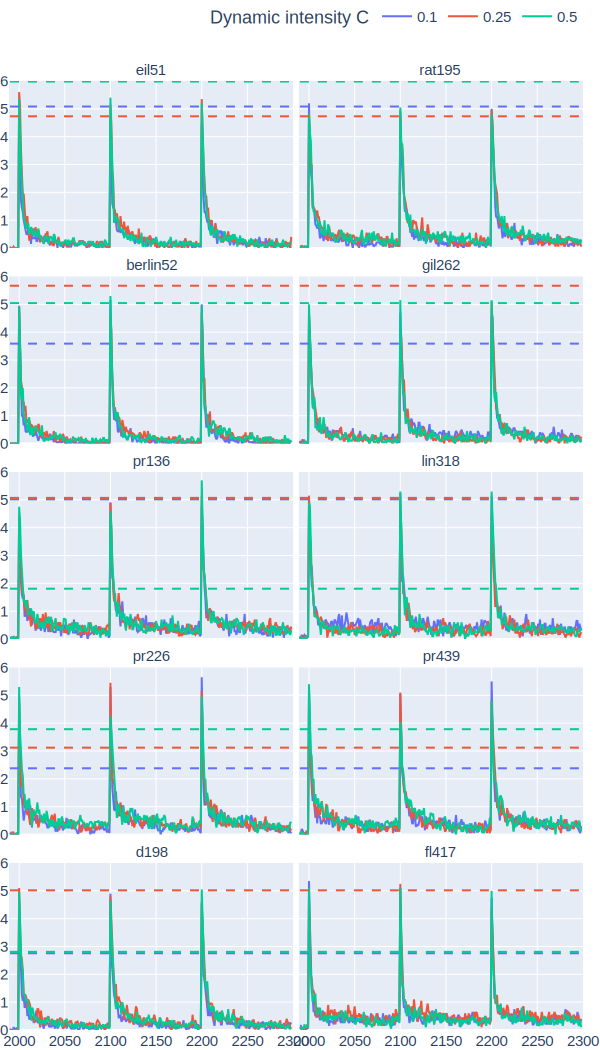
\includegraphics[width=0.725\textwidth]{results/part3/run_plot_cmp_dynamic_aggr_problem_y_swaps_1_to_30_HPO.svg}
	\caption[Line plots showing the swaps within the \gls{sce} tree over dynamic iterations for the \gls{hpo} parameter set showing all three dynamic intensities $C$ with a plot for each \gls{tsp} instance.]{Line plots showing the relative solution quality swaps within the \gls{sce} tree over the first 300 dynamic iterations (starting just before iteration 2000) for the \gls{hpo} parameter set showing all three dynamic intensities $C$ with a plot for each \gls{tsp} instance. The smaller instances are in the left column and the larger instances are in the right column. Each row corresponds to the predefined structural groups (see \cref{fig:cluster-groups}).}
		\label{fig:run_plot_cmp_dynamic_aggr_problem_swaps_HPO}
	\end{figure}

Continuing with \cref{fig:run_plot_cmp_dynamic_aggr_problem_swaps_HPO}, which shows the swaps over the first three dynamic intervals, this time also separated by problem instance, and only for the \gls{hpo} parameter sets, we can also draw dashed line representing the dynamic threshold that triggers $H$. As before, the instances are arranged according to their structural group and dimension. 
Looking at the first three rows, the thresholds for at least two of the dynamic intensities are very high at around 5 swaps, or even 6 in the case of \texttt{eil51} and \texttt{rat195}, using $\theta = 0.460$ for the highest dynamic intensity $C=0.5$. This threshold is almost never reached, and even the two thresholds for the lower dynamic intensities are only just passed in some cases. Another interesting aspect in the third and fifth row is that here the \gls{hpo} process chose the lowest detection threshold for the highest dynamic intensity $C=0.5$ at $\theta_\text{pr136} = 0.139$ and $\theta_\text{d198} =  0.216$, which is consistent with the results from the previous discussion in \cref{chap:robustness}. 
Furthermore, the amount of swaps after the 50th iteration in each dynamic interval remains high as seen before, with the smallest instances, \texttt{eil51} and \texttt{berlin52}, reaching a lower value level than other instances, such as \texttt{lin318} and \texttt{rat195}, which show a much higher average amount of swaps in the later stages of the dynamic interval. Thus, even though the same parameter sets were used in each row for each dynamic intensity, either the higher dimension or influences of the city placement characteristic had an impact on the number of swaps within each structural group.


In addition to the number of swaps, two performance metrics from machine learning classification, also used in information retrieval, were calculated on the data. As explained in \cref{chap:an-part3}, these metrics are precision and recall. The precision describes how many detected iterations (\gls{tp} + \gls{fp}) were actually \gls{tp}, and thus describing how relevant the detected iterations are. The recall describes how many possible correctly detectable iterations (positives) were actually detected by the \gls{hsppbo} algorithm (\gls{tp}). Both metrics span a range between 0 and 1, where 0 means that no correct detections (\gls{tp}) were found at all, and 1 means that either every dynamic event correctly triggered the change handling procedure, but allowing for \glspl{fp} (recall), or that all change handling procedures triggered were in response to a dynamic event, but allowing for dynamic events without any response (precision). The direct results of these metrics can also be found in \cref{tab:detection-stats-all-hpo} for the \gls{hpo} parameter set and \cref{tab:detection-stats-all-ref} for the reference parameter set, both inducing each combination of \gls{tsp} problem instance and dynamic intensity $C$.

In \gls{ml} visualization, these metrics are often presented in precision-recall curves for certain thresholds of classification confidence. A very good classifier will have a $PR$ curve close to $precision=1$ for varying recall values. A common baseline in these plots is a line parallel to the recall axis for the precision value representing the fraction of all positives to all negatives, with a good classifier staying above this line. In an example with equal amounts of positives and negatives, this line is drawn at $precision=0.5$, thus a random classifier could achieve this precision on average. When applied to this problem, the dynamic detection threshold of \gls{hsppbo} is not comparable to a classifier threshold, making it impractical to draw a curve or area plot from these precision and recall values. Instead, scatter plots were drawn with the baseline at $precision=30/570\approx0.053$. 

\begin{figure}[h]
	\centering
	\begin{subfigure}[b]{1\textwidth}
		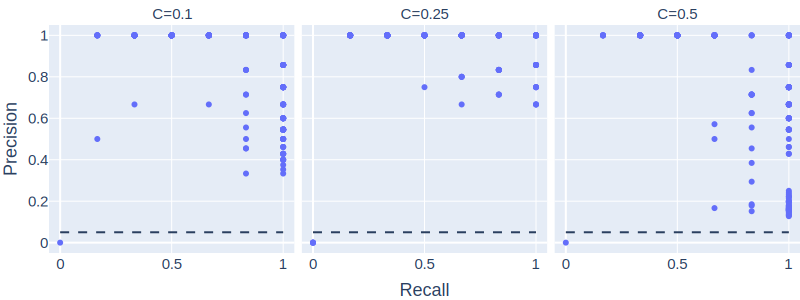
\includegraphics[width=1\textwidth]{results/part3/pr_curve_cmp_dynamic_grouped_False_HPO.svg}
		\caption{HPO}
		\label{fig:pr_curve_cmp_dynamic_HPO}
	\end{subfigure}
	\hfill
	\begin{subfigure}[b]{1\textwidth}
		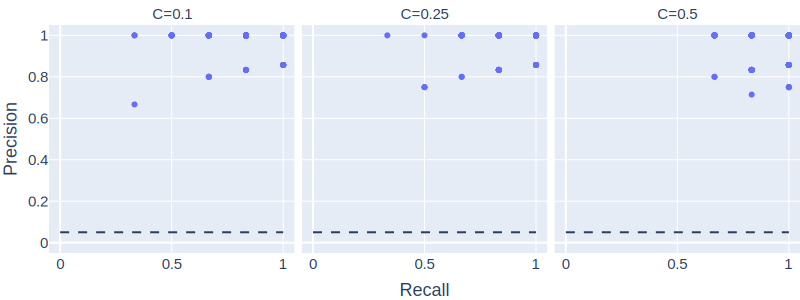
\includegraphics[width=1\textwidth]{results/part3/pr_curve_cmp_dynamic_grouped_False_Reference.svg}
		\caption{Reference}
		\label{fig:pr_curve_cmp_dynamic_Reference}
	\end{subfigure}
	\caption[Precision-Recall scatter plots separated by dynamic intensity $C$ for both parameter sets]{Precision-Recall scatter plots showing the values for recall on the x-axis and precision on the y-axis separated for each dynamic intensity $C$ (annotation at the top of the plots) for the \gls{hpo} (left) and the reference (right) parameter sets.}
	\label{fig:pr_curve_cmp_dynamic}
\end{figure}

\Cref{fig:pr_curve_cmp_dynamic} shows a $PR$ scatter plot for each dynamic intensity $C$, averaged over all \gls{tsp} instances, and compared for both the \gls{hpo} parameter set (\ref{fig:pr_curve_cmp_dynamic_HPO}) and the reference parameter set (\ref{fig:pr_curve_cmp_dynamic_Reference}). Again, the better dynamic detection performance of the reference set is clearly evident, with $PR$ points staying well above the precision baseline and mostly populating the upper right corner of the high precision and recall values, meaning that almost all dynamic events were found while avoiding \glsdesc{fp}. Interestingly, the performance on the least dynamic instances $C=0.1$ shows the worst $PR$ values at $recall = 0.33$ and $precision = 0.67$. This suggests that fewer dynamic events were detected in this case, which is to be expected since the static threshold of $\theta =0.25$ was reached less often. On the contrary, the highest dynamic intensity of $C=0.5$ showed the best $PR$ values.

Looking at the results for the \gls{hpo} parameter sets, the $PR$ values are more scattered, while generally performing worse, and sometimes coming close to the precision baseline. There even seemed to be multiple runs for all dynamic intensities where no dynamic events were detected ($PR = (0,0)$). 
The parameter sets for the medium dynamic intensity $C=0.25$ are able to obtain the best values for precision, when compared to the reference set. Although the highest dynamic intensity shows that many \gls{hsppbo} runs have detected all the dynamic events, reaching $recall =1$, the precision of these averaged runs was as low as $precision=0.13$. This indicates a very high amount of false detections (\gls{fp}) and thus false triggers of the change handling procedure. This is also partially true for the lowest dynamic intensity $C=0.1$, but the precision is slightly better, with the lowest value being $precision=0.33$, meaning that every third change handling procedure triggered was not a correct response to the dynamic event. This behavior could indicate that only in the case of medium dynamic intensity the \gls{hpo} considered a correct dynamic response as important enough for the goal of solution quality that it properly optimized for it. In contrast, especially with the choice of parameter values discussed before in mind (see \cref{fig:parameter_boxplot_dynamic}), the robust, high $\beta$ values for dynamic intensity $C=0.5$ and the robust, comparatively high $\alpha$ values for dynamic intensity $C=0.1$ suggest that for these dynamic environments, other parameters may be more important for good solution quality. This is also suggested in \cref{fig:parameter_importance_bar_dynamic}, although the higher importance of the detection threshold for $C=0.25$ lies in the error margin of the other two dynamic intensities.

\begin{figure}[h]
	\centering
	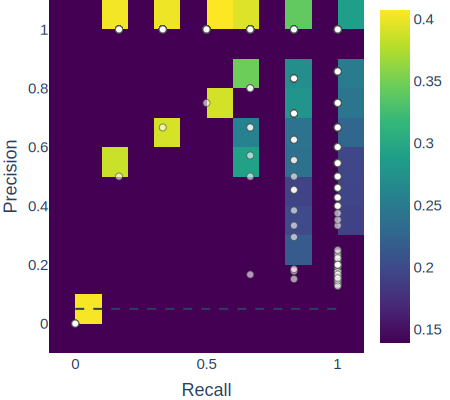
\includegraphics[width=0.55\textwidth]{results/part3/pr_curve_cmp_detection_threshold_grouped_True_HPO.svg}
	\caption[Precision-Recall heatmap showing the precision over the recall value with the z-axis displaying the detection threshold $\theta$ for the \gls{hpo} experiments]{Precision-Recall heatmap showing the precision over the recall value with the z-axis displaying the detection threshold $\theta$ as a color map for the \gls{hpo} experiments. The $\theta$ values for points in the same heatmap cell are averaged. In addition, the actual precision-recall points are overlayed to better seperate the darker areas.}
	\label{fig:pr_curve_cmp_detection_threshold}
\end{figure}

This relationship between high precision and recall values and the detection threshold seems to hold even more information about the dynamic detection capabilities of the \gls{hsppbo} metaheuristic. \Cref{fig:pr_curve_cmp_detection_threshold} shows the precision over the recall values, but with an underlying heatmap showing the detection threshold $\theta$ for the \gls{hpo} parameter set. Each heatmap cell represents the average $\theta$ value of all $PR$ points falling in that region, also called a bin. This is why the background appears to be covered by low $\theta$ values of 0.15, because this is the minimum value available for averaging and can be ignored if no point lies directly on that cell.
The worst performing runs with $PR = (0,0)$ used a very high detection threshold of $\theta \approx 0.4$, which requires 5 or more swaps in the \gls{sce} tree to trigger $H$. This value seems to be too high in almost all scenarios, because even the runs with $precision > 0.5$ using these high $\theta$ values only achieved suboptimal recall scores of $recall < 0.5$. This means that even though most of the $H$ triggers were correct responses to a dynamic event, more than half of the dynamic events went undetected. Looking at the near perfect upper right corner of $PR=(1,1)$, a dynamic detection value of $\theta = 0.29$ seems to be the best choice, which is very similar to the median seen in \cref{fig:parameter_boxplot}. While the recall remains high in the right section of the plot, the precision decreases with decreasing $\theta$ values.

Examining the $PR$ plot for each individual \gls{tsp} instance for the \gls{hpo} parameter set, shown in \cref{chap:figures} with \cref{fig:pr_curve_cmp_problem_HPO}, it appears that some instances achieved very good scores (e.g., the first two rows), while other instances had more problems with detecting dynamic events. However, this may very well be influenced by the parameters used rather than the problem instances themselves. Therefore, this visualization is not particularly significant and is only meant to further illustrate the effect of $\theta$ on the $PR$ scores.

\begin{figure}[h]
	\centering
	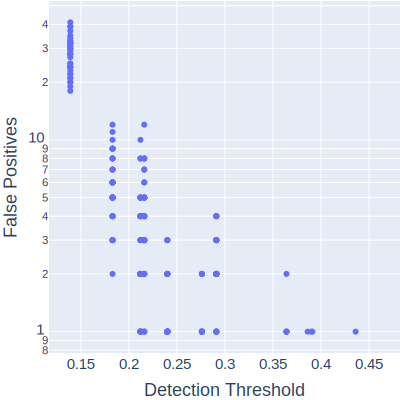
\includegraphics[width=0.5\textwidth]{results/part3/fp_theta_plot_HPO.svg}
	\caption[Scatter plot of all false dynamic detections by \gls{hsppbo} (\glsdesc{fp}) over the detection threshold $\theta$]{Scatter plot of all false dynamic detections by \gls{hsppbo} (\glsdesc{fp}) over the detection threshold $\theta$ for all 600 experimental runs using the \gls{hpo} parameter sets, using a logarithmic scale for the y-axis.}
	\label{fig:fp_theta_plot_HPO}
\end{figure}

Another interesting observation that proves that the dynamic detection works as expected is the relationship between \glsfirst{fp}, which are triggers of the change handling procedure that were not in correct response to a dynamic event, and the detection threshold $\theta$, shown in \cref{fig:fp_theta_plot_HPO}. A logarithmic y-axis was chosen because the \glspl{fp} increase exponentially with decreasing $\theta$. Therefore, we can clearly see an almost linear diagonal line from the upper left to the lower right of the scatter plot, suggesting that to greatly reduce false detections (to a fraction of $1/4$) from 40 to 10, we only need to slightly increase $\theta$ by 0.05 to $\theta = 0.19$,. However, any further reduction of \glspl{fp} can only be achieved by even higher increases in $\theta$ until a point is reached where we only have no false positives because we are not detecting anything at all.

\begin{table}[h]
	\setlength{\tabcolsep}{5pt}
	\centering
	\caption[The $F_1$ score averaged over all experimental runs for each combination of \gls{tsp} instance and dynamic intensity]{The $F_1$ score, i.e. the harmonic mean of the metrics precision and recall, and its standard error averaged over all $r_\text{exp} = 20$ experimental runs for each combination of \gls{tsp} instance (rows) and dynamic intensity $C$ (columns). Each element contains the values for the hyperparameter optimized parameters (\gls{hpo}, see \ref{tab:best-parameters}) and the reference parameter set (see \ref{tab:part3-gen-params}).}
	\label{tab:detection-stats-f1}
	\begin{adjustbox}{width=1\textwidth}
	\begin{tabular}{l  S[round-precision=2,table-format=1.2(2)] S[round-precision=2,table-format=1.2(2)]  S[round-precision=2,table-format=1.2(2)] S[round-precision=2,table-format=1.2(2)]  S[round-precision=2,table-format=1.2(2)] S[round-precision=2,table-format=1.2(2)]  S[round-precision=2,table-format=1.2(2)] S[round-precision=2,table-format=1.2(2)]}
		\hline
		 \gls{tsp} & \multicolumn{2}{c}{$C=0.10$} & \multicolumn{2}{c}{$C=0.25$} & \multicolumn{2}{c}{$C=0.50$} & \multicolumn{2}{c}{$\overline{C}$} \\ 
		 \cmidrule(lr){2-3} \cmidrule(lr){4-5}  \cmidrule(lr){6-7} \cmidrule(lr){8-9}
		~ & \text{HPO}  & \text{Ref.} & \text{HPO} & \text{Ref.} & \text{HPO} & \text{Ref.} & \text{HPO} & \text{Ref.}\\ \hline
		eil51 & 0.56(0.05) & 0.88(0.02) & 0.89(0.03) & 0.91(0.02) & 0.65(0.03) & 0.96(0.01) &0.70(0.03)& 0.92(0.01)\\
		rat195 & 0.63(0.04) & 0.89(0.02) & 0.86(0.02) & 0.94(0.01)  & 0.65(0.03) & 0.94(0.01) &0.71(0.02)&0.92(0.01)\\ \hline
		berlin52 & 0.92(0.01) &0.84(0.03)& 0.57(0.05) &0.95(0.02)& 0.59(0.05) & 0.93(0.02) &0.69(0.03)& 0.91(0.02)\\
		gil262 & 0.89(0.03) & 0.91(0.02) & 0.55(0.05) & 0.88(0.03)  & 0.66(0.04) &  0.96(0.01) &0.70(0.03)&0.92(0.01)\\ \hline
		pr136 & 0.61(0.04) & 0.89(0.02) & 0.56(0.05) & 0.92(0.02) & 0.27(0.01) & 0.96(0.02)  &0.48(0.03)&0.92(0.01)\\
		lin318 & 0.67(0.03) & 0.87(0.03) & 0.59(0.04) &  0.94(0.01) & 0.32(0.01) & 0.94(0.02)  &0.53(0.03)&0.92(0.01)\\ \hline
		pr226 & 0.66(0.01) & 0.91(0.02) & 0.88(0.02) & 0.91(0.02) & 0.84(0.03) & 0.94(0.02) &0.79(0.02)& 0.92(0.01)\\
		pr439 & 0.68(0.02) & 0.95(0.01) & 0.89(0.02) & 0.92(0.01) & 0.84(0.02) & 0.93(0.02) &0.80(0.02)& 0.93(0.01)\\ \hline
		d198 & 0.87(0.02) & 0.96(0.01) & 0.58(0.03) & 0.91(0.03) & 0.76(0.02) & 0.91(0.02) &0.73(0.02)&0.93(0.01) \\
		fl417 & 0.75(0.02) & 0.90(0.02) & 0.47(0.04) & 0.91(0.02) & 0.76(0.04) & 0.92(0.02) &0.66(0.03)& 0.91(0.01)\\ \hline
		$\overline{\text{\gls{tsp}}}$ & 0.72(0.01) & 0.90(0.01) & 0.68(0.02) & 0.92(0.01) & 0.63(0.02) & 0.94(0.00) &0.68(0.01)& 0.92(0.00)\\ \hline
	\end{tabular}
	\end{adjustbox}
\end{table}

Finally, all of the precision and recall values are combined into a harmonic mean, the so-called $F_1$ score, which is high, if both precision and recall are good, while a low $F_1$ score indicates poor performance in at least one of these aspects. It is particularly useful when the two metrics are of equal importance, as is the case here. The score is shown in \cref{tab:detection-stats-f1} for each combination of \gls{tsp} instance and dynamic detection threshold $C$, their respective means $\overline{\text{\gls{tsp}}}$ and $\overline{C}$, compared between the \gls{hpo} parameter sets and the reference set, with additional standard error from averaging. Each pair of rows separated by a line represents a structural group.

The data shows better dynamic detection by the reference parameter set than the \gls{hpo} sets in almost every direct comparison. Even more impressive, the reference value of $\theta = 0.25$ achieves values of $F_1 \geq 0.9$ in almost every combination of problem instance and dynamic intensity, with a total average over all values of $F_{1_\text{Ref}} = 0.92$. The total average of the \gls{hpo} parameter sets is 26\% lower at only $F_{1_\text{HPO}} = 0.68$. 
Only a few combinations of \gls{tsp} instance and dynamic intensity, and therefore specific parameter sets, were able to achieve satisfactory results. These exceptions are the first structural group with $C=0.25$ using a $\theta = 0.364$, the second structural group with $C=0.1$ using $\theta = 0.276$, the fourth group with $C=0.25$ using $\theta = 0.240$, and the fifth group with $C=0.1$ using $\theta = 0.212$. However, these exceptions are still worse than the scores in the same category obtained by the reference set, except for the second structural group, specifically \texttt{berlin52} with $C=0.1$, where $\theta = 0.276$, resulted in a $F_1$ score slightly better than that of the reference set.

In summary, the dynamic detection of the reference set using $\theta = 0.25$ almost always outperforms the parameter sets acquired by \gls{hpo}. This suggests that by using only the solution quality as a metric for the response to dynamic changes, the \gls{hpo} process, or at least the chosen \gls{gbrt} method, generally does not evaluate the correct dynamic detection as relevant to the search process, and thus, as expected in hindsight, values good solutions above all else. The superior solution quality has already been discussed before, leaving no doubt about the success of the \gls{hpo} process in that regard. However, it appears that unless the correct response to dynamic changes is explicitly made a requirement in the scoring function $f(\lambda)$, the process will not automatically include this goal in its search for well-performing parameters. The question then becomes whether this is even necessary if the solutions to the \gls{dtsp} are still remarkably good.